\documentclass[12pt]{article}
\fontfamily{times}
\usepackage{url}
\usepackage[margin=1in]{geometry}
\usepackage{array}
\usepackage{ragged2e}
\usepackage[utf8]{inputenc}
\usepackage[T1]{fontenc}
\usepackage{fullpage}
\usepackage{parskip}
\usepackage{titling}
\usepackage{tikz}
\setlength{\parindent}{15pt}
\usepackage{times}
\usepackage{booktabs}
\usepackage{longtable}
\usepackage{siunitx}
\usepackage{graphicx}
\usepackage{amsmath}
\usepackage{authblk}
\usepackage[american]{babel}
\usepackage{csquotes}
\usepackage[hidelinks]{hyperref}
\usepackage[authordate,backend=biber]{biblatex-chicago}

\addbibresource[location=remote]{https://virginia.box.com/shared/static/m0nw01c4bcltkauwy2hd1467vu7dufrj.bib}
\usepackage[section]{placeins}

\author{Robert Kubinec and John Owen}
\affil{\small Department of Politics \\
	\small University of Virginia}
\date{\small \today}

\linespread{1.5}

\title{Islamist-Secularist Protest during the Arab Uprising}

\begin{document}

\maketitle

	\begin{abstract}
		Scholars continue to disagree as to how far contentious politics diffuses within and across states and by what mechanisms it does so. We use new data and empirical measures to test polarization during and after the Arab Uprisings of 2010-12. After authoritarian governments began to fall, populations in several states began to polarize between secularists and Islamists over what kind of regime was to replace the ousted one. We hypothesize that this Islamist-secularist polarization was triggered by catalytic events (such as the military's coup against the Muslim Brotherhood in Egypt) and diffused transnationally owing to social media and satellite television, dividing anti-status-quo actors throughout the region. To examine polarization over time, we collected a comprehensive dataset on elite and citizen Twitter accounts across Arab countries after the Arab Spring. Using item-response models, we model polarization as the difference in latent ideological position between elites while accounting for feedback effects, and we show how polarization within countries changes over time in response to exogenous political shocks. By doing so we are the first to offer compelling statistical evidence of the endogenous process of polarization across competing ideological groups and states.\footnote{\linespread{.5} We thank Steven Livingston and meeting participants at the 2017 American Political Science Association Annual Conference for valuable criticism. The authors thank the Amb. Henry J. and Mrs. Marion R. Taylor Chair at the University of Virginia for research funding.  John Owen thanks the Liu Institute for Global Inquiry at the University of British Columbia for providing a research venue. Robert Kubinec thanks the University of Virginia's Quantitative Collaborative for computing resources and Jonathan Kropko for helpful feedback on this project.}
	\end{abstract}

	\section*{Introduction}

	The Arab Uprising of 2010-13 was an exceedingly complex phenomenon.  The initial event – the self-immolation of Mohamed Bouazizi in Sidi Bouzid, Tunisia – triggered a chain of events marked by interaction and feedback loops.  During the Uprising, experts predicted a particular unfolding or winding down of the phenomenon, and often were wrong.  Some assured their readers that the Tunisian unrest of December 2010 and January 2011 would not spread to other Arab countries (Karon 2011; Walt 2011); others predicted that the unrest that did spread to Libya, Egypt, Yemen, Syria, and elsewhere would bring liberal democracy to those countries (Obama 2011, Jupp\'{e} 2011).  In other words, two of the unpredictable developments were the spread of unrest across countries and the evident shift in the goals of rebels.  
A helpful approach to explaining, if not predicting, the progress of the Arab Uprising and infectious political unrest more generally is via group polarization, or the endogenous segregation of a population by preferences into two or more mutually antagonistic groups.  

Group polarization is situational and hence may be short-lived; it is different from the long-term, materially based social polarization that many social scientists study (Moulaert et al. 2003).  Group polarization is a way to conceive of how identities and preferences change in response to exogenous events such as a public demonstration or a coup d'\'{e}tat.  A stylized version runs as follows:  At time $t$, an unmodeled event takes place (e.g., Bouazizi's self-immolation); at $t+1$, the news spreads; at $t+2$, a portion of the population of Sidi Bouzid becomes angry and identifies more strongly against the local and national government, as reflected in anti-government speech and action; at $t+3$, news of that speech and action spreads; at $t+4$, a portion of Sidi Bouzid's population becomes angry at the protesters and identifies more strongly with the government, as reflected in pro-government speech and action; at $t+5$, news of that speech and action spread within Tunisia and beyond; and so on.  Group polarization is self-reinforcing.  It may be slowed, halted, or reversed by various developments, including coercion (censorship, physical force) by governments.

Its situational quality, specifically its dependence on exogenous events, makes group polarization impossible to predict, but therefore especially helpful in understanding complex chains of events such as the Arab Uprising.  The group-polarization approach presupposes, with a long tradition in social theory, that people have multiple group affiliations; that belonging to one group entails defining oneself over against one or more alternative groups; that for a given individual at a given time a particular group affiliation may be more or less salient; and that individuals respond to signals of friendship and hostility from one another; and hence that populations sometimes polarize along one axis of identity, temporarily submerging other axes of identity.  Of particular interest in the Arab Uprising are (1) cross-polarization, or the shift from polarization along one axis (e.g., pro- versus anti-regime) to polarization along a cross-cutting axis (e.g., Islamist versus secularist), and (2) transnational polarization, i.e., simultaneous polarization along an identity axis in two countries.

Group polarization is a phenomenon of changing sentiment, identity, and preference.  Measuring it with rigor has been difficult, and thus so has testing claims about what triggers it and what suppresses it.  The growing use of social media, the availability of the resulting data, and advances in computing power, however, combine to allow researchers to measure changes in group polarization over time.  In this paper, we present analysis of Twitter data during 2013 in Egypt and Tunisia.  We choose this time period because Egypt went through a number of political events that seem prime candidates for triggers of group polarization.  Most obvious is the July 3 coup d'état in which secularist military officers overthrew the elected government of Mohamed Morsi of the Muslim Brotherhood.  Other potentially polarizing events include clashes between Muslims and Christians in al-Khousos on April 6-7; Morsi's appointment of seven new governors from the Muslim Brotherhood on June 16; and the military government's violent dispersal of pro-Morsi demonstrators in Cairo on August 14 (Daily News Egypt, https://dailynewsegypt.com/2013/08/14/live-updates-pro-morsi-sit-ins-dispersed/, retrieved on 11 August 2017.) 

This paper presents a Bayesian item response theory model that incorporates feedback loops between ideological groups through the use of co-integrated time-series priors on latent constructs. The item response theory model has been widely used to study social and group polarization, but we are the first to show how to explicitly model feedback by proposing that similar cross-country ideological groups will tend to show auto-correlated trends over time. In other words, we expect that the differences between the ideological positions of secularists in Egypt and secularists in Tunisia will be roughly proportional (i.e., stationary) over time, while the same condition will hold for Islamists in both countries. 

In what follows, we explicate the logic of group polarization in an informal model.  We include propositions about de-polarization and cross-polarization.  We offer hypotheses about group polarization, and explain and defend our use of tweets in Egypt and Tunisia in 2013.  We present the statistical model and data analysis.  We close with thoughts for future research.


\section*{Group Polarization: An Informal Model}
Polarization has been studied extensively by social scientists.  Much of that work concerns social polarization, or segregation into groups that are stable over long periods of time (such as ``Red America" and ``Blue America").   By group polarization, we mean a process of segregation – not an equilibrium – that is relatively short-term or situational yet may be politically consequential.   Along with other scholars, we define polarization as a social construct, namely as progressive identity change that entails preference change.   When two actors polarize, at time $t$, both actors may prefer a 50-50 allocation of goods; at $t+1$, each may prefer a 60-40 allocation in its favor; at $t+2$, a 75-25 allocation; and so on.  At the limit of polarization, each side wishes the other destroyed.   Group polarization, then, is one way to formulate a progressive worsening of conflict; it does not cause conflict, in the sense of an independent variable causing a dependent one.  Rather, polarization is conflict that is self-intensifying.  Group polarization is endogenous, not in the sense that it is unrelated to pre-existing cleavages bur rather in the sense that, once triggered by exogenous events, it is self-intensifying.   It entails the altering of individuals' preferences and practices and creates new threats and opportunities for various actors, including actual and aspiring rulers (Owen 2015: 55-61)..  

Stated informally, the basic group polarization model is simple.  Assume a population of 100 persons, all 100 belonging to one half or another of $x$ pairs of opposing social groups (labor or capital, democrats or authoritarians, Islamists or secularists, urban or rural, etc., etc.).  Fifty are pro-democracy, fifty pro-authoritarian.  These groups do not correlate significantly to any other groups; e.g., democrats are as likely to be Islamist as secularist.  The population thus has cross-cutting cleavages.   At time $t$, the population begins in an unbiased equilibrium, such that, although individuals may identify more strongly with one group affiliation than with others, in the population as a whole, no identity axis predominates; hence social interaction does not skew the distribution of resources, including information, to any of the social groups (Dunning and Harrison 2010).  Now suppose that at $t+1$ three democrats – one Islamist and two secularist, and two urban and one rural – publicly beat an authoritarian.  Assuming a relatively free flow of information, that event can trigger the polarization of the population along a democratic-authoritarian ideological axis, such that democrats and authoritarians care less and less about class, being urban or rural, or mosque-state questions and more and more about ideology.  If not disrupted, polarization by definition culminates in inter-group violence.

Transnational group polarization takes place when polarization spans two or more countries at once.  Citizenship in a state amounts to yet another group affiliation, albeit normally an especially politically salient one that carries the advantages of a state apparatus.  States are set up to foster group identity and loyalty vis-à-vis foreigners.  They may use physical segregation, closed or semi-closed national borders, national economic integration, propaganda, history, threats of war, coercion, and other means to induce a strong national identity among citizens and hence a strong sense that foreigners are an ``other."  Yet, interaction – communication, trade, investment, travel – across state borders is normal, particularly among most countries in the twenty-first century.   States vary in their capacity to build and maintain a national identity and to have that identity perpetually trump all other group affiliations, including transnational ones, across all conditions.   Thus transnational group affiliations – ethnic, religious, ideological, class, sexual – are part of life for people in most countries.  Insofar as communication across state boundaries is uncensored by states, transnational group affiliations can yield transnational group polarization.  The informal model above may then incorporate democrats and authoritarians in a second state (and a third, a fourth, and so on).

Cross-polarization takes place when a group at time $t-1$ is not in unbiased equilibrium, but instead is polarized along one identity axis and at t an event triggers polarization along a different axis.  In the example above, at t the population is segregated according to preference into Islamists and secularists.  At $t+1$, three authoritarians (say, one Islamist and two secularist) publicly beat a democrat.  At $t+2$, as Islamists and secularists who are democrats begin to identify more as democrats and less as Islamists or secularists.  Polarization of the entire population along a democrat-authoritarian axis will commence.

Group de-polarization – understood as a diminution of speech and acts biased according to group affiliation – may set in when communication is censored or degraded or speech and action forcibly curtailed.  The most obvious agent of de-polarization is a government, which typically has at least some of the means of censorship and coercion at its disposal.  A government threatened by polarization into pro- and anti-government groups can be expected to try to slow, halt, or reverse it – or to trigger a cross-polarization that would weaken the anti-government group.  

\section*{Justifying Assumptions}
Social identity theory links the formation of groups and their degree of competition by means of the concept of polarization.  Microfoundations for such a model are in philosophy and social theory.  Assume that persons are not atomized individuals whose fundamental goal is to maximize their own exogenously derived utility and who value the gains and losses of others only insofar as those are instrumental to such maximization.  Assume instead the persons depicted by traditions in sociology (Simmel 1955; Coser 1956):  each individual is fundamentally a member of social groups, and he identifies his interests to some extent with those of the groups to which he belongs and against opposing groups.

The logical foundations of this communal psychology is seen in the formula articulated by Spinoza and, later, Hegel:  omnis determinatio est negatio, or ``all determination is negation" (Melamed 2013).  A thing must necessarily have properties, such as ``short" or ``cold."  But properties only exist in contrast to other properties (Taylor 1975, 232-39).  Human being contrasts to non-human being (animals, plants, rocks); female, to male; labor, to capital; old, to young; and so on.  Having a self requires having an other.   Having a property is equivalent to belonging to the set of things that have that property (Quine 1989, 22-26).  Being female is equivalent to being a member of the set of persons that are female.  Identity thus is social:  who I am entails my group memberships.

Philosophers may disagree on the soundness of this logic, but experimental evidence suggests that people, or at least some people, tend to think, feel, and act according to it.  People tend to be self-interested, but their notion of ``self" may expand to include persons in their social group whose existence requires contrast with some opposing or ``out-group" (Mercer 1995).  Indeed, these two identifications are mutually constitutive.  As Simmel put the matter,
\begin{quotation}
	``It appears to be necessary for us human beings, whose whole psychical nature is built upon our sensitiveness of difference, that a feeling of separateness should always exist alongside of the feeling of unity to make this latter perceptible and tangible" (Simmel 1898, 45-46).  
\end{quotation} 

\section*{Overlapping Social Groups and Different Saliencies}
That individuals belong to multiple social groups, each with a corresponding anti-group, introduces a complication.  For Simmel, an individual's identity consists of the unique overlap of the groups to which she belongs (Simmel 1955, 139-41).  Yet, a given individual will identify more strongly with some of his groups than with others.  
Sometimes large groups of individuals do so simultaneously, such that populations polarize along a particular axis of group identity.   Social-psychological literature posits at least two attributes of groups that lend them high salience.  One is prestige or high status:  experiments show that members of high-status groups are significantly more biased toward fellow members and against nonmembers than are members of low-status groups.   Experiments also show that a second attribute is threat (physical, economic, status, etc.) – particularly among persons already highly committed to the group (Ellemers et al. 2002).  A new threat – such as an attack on a group member by members of the opposing group – tends to arouse in such persons fears that they may be next, and so they tend to increase their biases toward that particular group affiliation.  They identify more with it and against the threatening group.  This experimental result is anticipated by Simmel:

\begin{quotation}
	``It is a fact of the greatest social significance, one of the few which are true almost without exception of group formations of every sort, that common antagonism against a third party under all circumstances tends to consolidate the combining group, and with much greater certainty than community in friendly relationships toward a third party" (Simmel 1898: 45-46).
\end{quotation}


If these attributes of prestige and threat are associated with high salience, it should be the case that a rise in a group's status or endangerment can render it more salient for its members.  A rise in status may be triggered in politics by a victory in an election or a civil war, or an unexpectedly large public rally.  A rise in threat may be brought on by physical violence, verbal abuse, or evidence of discrimination or persecution against the group.

Social-psychological literature notes that people vary by level of commitment to various groups.   In equilibrium some city-dwelling Islamists identify more as urban and less as Islamist; others identify more as Islamist as less as urban.  This kind of heterogeneity could in principle stifle polarization, because low-commitment group members could try to exit or hide from the group rather than take the risks that come with strongly identifying with it.  Against that possibility, Tilly writes that, following a triggering event, highly committed group members mediate and broker polarization by spreading information about the threat or increased status and about ongoing polarization.   Such brokers may propagandize by exaggerating and inventing symbolic events.  Public discourse turns to what is to be done; those who hold extreme views tend to have more influence in such times and moderates either are quiet or move toward the extreme (Tilly 2005, 143-44).   Smith (2012) models allocation decisions in a game comprising two social groups, each comprising two types of actors:  ``behavioral" actors who are biased to favor their own group members, and ``rational" actors who are unbiased.  The model shows that ``rational" across will come to act like ``behavioral" ones and favor allocation of goods to their own group.  

It stands to reason that the low-commitment actors posited by Ellemers et al. would behave like Smith's ``rational" actors.
In sum, an exogenous event that either raises the prestige of social group $A$ or threatens group $A$ may cause people who belong to multiple overlapping groups $A$ through $Z$ to identify more strongly with $A$ and against $\neg A$ and less with $B$ and against $\neg B$, etc.  Increases in status and in threats may be simultaneous:  an increase in $A$'s status may simultaneously threaten members of $\neg A$ and thus cause them to identify more as $\neg A$s and against group $A$.  Large public anti-government demonstrations, as take place during a typical political spring, can both raise the status of being anti-government and simultaneously threaten those who identify with the government.  And again, polarization tends to feed on itself:  as members of $A$ observe members of $\neg A$ identifying more as $\neg A$s, members of $A$ will identify still more strongly with $A$; and so on. 

\section*{Hypotheses}

We propose to test the following hypotheses based on this theory:

\begin{tabular}{lp{15cm}}
	H1 & After polarizing events, the difference in latent ideological positions between competing groups will diverge from each other very quickly.\\
	H2 & After polarizing events, cross-national ideological groups will tend to increase within-country polarization in response to events occurring in the other country.\\
	H3 & After polarizing events, ideological groups in other countries will become more sensitive to changes in the position of their like-minded actors in other countries.
\end{tabular}

We can operationalize these hypotheses by estimating ideological position as a latent ideal point that can vary over time. For these reasons, we collected data on ideological actors in Egypt and Tunisia from Twitter, as we described in the next section. For hypotheses 2 and 3, we need to have summary statistics that look at patterns of ideological interaction across countries and see if these summary statistics change as a result of the polarizing event of interest. 

The primary event we are most interested in is the coup that overthrew President Mohammed Morsi in July of 2013 as it represented a clear division between secularists and Islamists. Other polarizing events occurred during this period and previous to our period of data collection, but we focus our attention on the coup because it represents the event of highest salience, representing full forced regime change that removed Islamists from power and ended democratization in Egypt.
 
\section*{Data Collection}
Analyzing these phenomena quantitatively is difficult because we need good measures of ideology across countries that also varies over time. The advent of social media during the Arab Uprisings provides some of the first available data that we can use to examine the predictions of the theory. We chose to use Twitter due to its public nature and the ability to closely track elite users, or those users with a large number of followers. We built a sample of Egyptian and Tunisian twitter users that are broadly representative of political thinking \& discourse within these countries.

To obtain the sample, we started with a universe of tweets from the early stage of the Arab Spring, December 2010 to April 1st, 2011 that all matched the search times ``Cairo", ``Alexandria" and ``Tunis" in the location field in Twitter.  This dataset of 11 million tweets was then parsed in order to identify users that had received the largest number of retweets and mentions during that time period. We curated the resulting list of elite users, both by removing accounts that were later abandoned and by adding ideological diversity. In general, Twitter in 2011 was dominated by well-educated secular elites with a flair for democracy, while Islamists and pro-regime figures were later to adopt Twitter as a medium. For example, in Egypt we added the account for Mohammed Morsi, the Islamist president affiliated with the Muslim Brotherhood, and in Tunisia we added Rached Ghannouchi, long considered to be the guiding force of the Islamist Nahda movement in Tunisia. The full list of users selected for analysis is available in the appendix.

The final sample amounted to 142 Twitter users, 50 from Tunisia and 92 from Egypt. The larger number from Egypt reflects the much larger Twitter-sphere in the country and hence the need to obtain a broader sample of users. We then had two graduate assistants code the user list along two axes: Islamist-Secularist and Pro/Anti Democracy. We found both Islamists and secularists who were pro and anti-democracy, which we diagnosed by whether the elite was willing to oppose their own ideological allies when democratic norms were threatened by their own group, such as secularists opposing the coup that overthrew Mohammed Morsi. For that reason, these cleavages can be considered distinct, although in general we found it harder to identify pro and anti-democratic views because of the strong normative bias against expressing pro-authoritarian discourse. 

We focus on the Islamist-secularist distinction in this paper because there are more observable indicators for this cleavage during the time period in question, such as tweets supporting or opposing the Muslim Brotherhood, in addition to the fact that adding an explicit second dimension would make the ensuing model far more complicated, although we return to this issue in the discussion. In addition to these binary classifications, we also had the graduate coders record their confidence in their assessment on a scale of 0 to 100. We further reviewed cases that had an uncertainty of less than 50 percent. In general, these users did not tweet as much on political topics and their ideology is relatively unknown. We excluded these users for the analyses we report here as their lack of ideological content makes them uninteresting to this analysis.

With this finished list of 142 elite users, we then collected their full tweet histories from March 31st, 2013 to December 31st, 2013. This 1.7 million list of tweets was then filtered down to 1.2 million tweets that constitute each user's own composed tweets by removing all of each user's retweets. Using Twitter's open API, the retweets of all of these 1.2 million original tweets was then downloaded as a list of user IDs for each user per day for a total of 275 days. The use of the open API represents a limitation in the data collection because only 100 re-tweets of a given retweet may be downloaded; however, this limit was rarely reached in practice because very few of the tweets in question had more than 100 retweets. Even ex-President Mohammed Morsi, who has more than a million twitter followers, averaged only a few hundred re-tweets per tweet during 2013. Nonetheless, this data must still be understood as a sample of the full number of retweets, especially for users with a very large popular following.

The final database comprises a set of elites $j$ and citizens $i$ in which the outcome is the number of times that $i$ retweeted $j$ for each three-day in the sample. Three-day periods were chosen because it helps to address weekend seasonality (any particular period could fall on any part of the week), and because it results in a reasonable 92 time points in our sample. We took these retweets and we calculated how many times a specific user/citizen retweeted each elite within the three-day window. We then appended this data together for all the elites in our sample, comprising a dataset of 396,256 citizen-elite pairs.\footnote{We also had to sample 500 tweets from the Egyptian collection for each period in our sample due to the massive size of the remaining tweets and lengthy processing times.} We removed all citizens who did not re-tweet at least three different elites during the entire time period, resulting in a final dataset of 180,321 citizen-elite pairs with a total of 18,107 unique citizen Twitter users, or an average of 10 retweets per user. We do not include zeroes in the dataset for periods when a user did not re-tweet an elite because we do not know if a user saw a tweet and chose not to re-tweet or whether they never saw the tweet in question. For that reason, we would prefer to include only observed data in the model, while making the assumption that users would be equally likely to re-tweet similar ideological elites conditional on the users seeing these tweets.

The set of elites is further divided into four groups based on the RA coding: Islamists in Egypt and Tunisia versus secularists in Egypt and Tunisia. We can then think of each group having an average position in an ideological ideal point space that varies over the number of days in the sample. We do not account for the pro- and anti-democracy axis, so for that reason these estimates implicitly average over this cleavage within ideological groups.

\section*{Modeling Ideological Polarization Over Time}
To adequately model these phenomena, we combine two distinct literatures in statistics: time-series econometrics, in particular co-integrated equations, with the item-response theory literature on estimating latent concepts. Item-response theory has been used in political science for estimating the latent positions of actors based on roll-call voting datasets \parencite{jackman2004}, and more recently, through social media and campaign finance contributions \parencite{bonica2014,barbera2015}. Item-response theory (IRT) has also been applied to difficult measurement problems, in particular the construction of democratization indices from a variety of coding sources \parencite{vdem2017,treier2008}. Item response models estimate latent traits for individual cases that can be divided into two distinct groups, such as raters and countries, lawmakers and bills, or in our sample, citizens and elites. 

What is crucial about these models is that the latent estimates are unobserved. For that reason, there is a strong connection between IRT and factor analysis \parencite{takane1986}, and similar concerns over the interpretation of the latent scores are justified. The latent dimension estimated by an IRT model will be the lowest-variance explanation of the observed data, but further prior knowledge and post-estimation validation is necessary to confirm that the results correspond with the concept of interest. We are confident in our application of this technique to the data because of our prior coding of users into similar ideological groups. For that reason, the resulting estimates will reflect these latent cleavages instead of arbitrary social behaviors or groupings.

The application of time series modeling to IRT is more limited despite the fact that political science has many time-varying variables with considerable measurement error. This paper builds on the approaches of \textcite{quinn2002} and \textcite{kropko2013} who use random-walk priors on latent-traits to incorporate change in ideal points over time. In time-series lingo, these latent traits become integrated variables that exhibit an infinite memory process: any shifts in the ideal points are remembered in the time series over time \parencite[Ch. 5]{timeseries2014}. This assumption is safe for ideological constructs because we often do not imagine ideology reflecting stationarity, i.e., that ideologies receive random shocks that cause diversion and eventual return to an equilibrium \parencite[Ch. 2]{timeseries2014}. Rather, ideological polarization over time should move in a continually-changing direction as human beings adapt and respond to changing environmental conditions \parencite{owen2010clash}. For this reason, we do not adopt the approach of \textcite{park2011}, who models ``preference regimes" as showing stasis over time with brief moments of change in a form of punctuated equilibrium.

In addition to examining change over time, our research explores transnational ideological polarization. We want to know whether an increase in Islamist-secularist polarization in Egypt causes changes in Islamist-secularist polarization in Tunisia. This theory that we explicated informally corresponds most closely to the the idea of co-integrated time series. A co-integrated series involves two integrated or random-walk time series that exhibit a stationary relationship over time \parencite{engle1987}. Formally it can be defined as follows: given two integrated time series  $y$,

\begin{equation}
	y_t = y_{t-1} + \epsilon_{yt}
\end{equation}

and $x$,

\begin{equation}
x_t = x_{t-1} + \epsilon_{xt}
\end{equation}

we propose that these series are co-integrated as a linear combination through the parameters $\beta_1$ and $\beta_2$ such that the following identity holds true:

\begin{equation}
z_t = \beta_1 y_t + \beta_2 x_t + \epsilon_{zt}
\end{equation}

Where $z_t$ represents the relationship between $y_t$ and $x_t$ that is stable (stationary) over time and $\epsilon_{zt}$ is a white-noise error term \parencite[253]{engle1987}. Thus while both $x_t$ and $y_t$ follow a random walk, the existence of $z_t$ ensures that they will co-evolve. Furthermore, the parameters $\beta_1$ and $\beta_2$ determine the direction of feedback, i.e., how much feedback $y_t$ receives from $x_t$ and vice versa. In time series parlance they are known as the ``co-integrating vector", and usually one $\beta$ is fixed at 1 as otherwise the two parameters are un-identified \parencite[253]{timeseries2014}. 

We can then combine these ideas into a two-equation co-integrating equation model in which $x_t$ and $y_t$ are functions both of their previous values and of a feedback process from each:

\begin{align}
 y_t =& y_{t-1} + \gamma (y_{t-1} - \frac{\beta_2}{\beta_1}x_{t-1}) + \epsilon_{yt}\\
  x_t =& x_{t-1} + \gamma (x_{t-1} - \frac{\beta_1}{\beta_2}y_{t-1}) + \epsilon_{xt}
\end{align}

While co-integrated models are generally estimated in differences, we do not care about the differenced version of latent ideological positions, and so the model becomes somewhat simpler. The scaling parameter $\gamma \in (0,1)$ governs the degree of co-integration in the model: when $\gamma$ is high, the two time series will follow each other closer, but when $\gamma$ is small, the series are only marginally co-integrated. Furthermore, if we fix $\beta_1$ at 1, then a value of $\beta_2$ greater than 1 signifies that $y_t$ sends more influence to $x_t$ than $x_t$ sends to $y_t$. 

To apply this form of feedback process to IRT, first consider the standard 2-PL IRT model that is identical to the canonical ideal point model in political science \parencite{jackman2004}:

\begin{equation}
Y_{ij} = \prod^{i=1}_I \prod^{j=1}_J \phi(\delta_j * \alpha_i - \eta_j)
\end{equation}

In this model, $\alpha_i$ represent the latent ideal points of the elites, while $\delta_j$ represent discrimination parameters for each citizen (equivalent to factor scores) and $\eta_j$ can be interpreted as the average probability that citizen $j$ retweets elite $i$ $Y_{ij}$ times. Given that in our data the number of re-tweets of a particular elite $i$ has a maximum of three for each period, we use an ordered-logistic function $\phi(\cdot)$ for $Y_{ij}$ that estimates cutpoints $c_{ijk}$ for each retweet $k \in K$ with a maximum of $K=3$.\footnote{For a full explication of the ordinal IRT model for ideal points, see \textcite{kubinec2017}.}

For our purposes, we have four $\alpha_i$ parameters that represent each of our ideological groups, so we can subscript them as $\alpha_{ig}$ where $g \in [1,2]$ cleavages (Islamist, Secularist) and $i \in [1,2]$ countries (Tunisia, Egypt).  Building on \textcite{quinn2002} and \textcite{kropko2013}, we can include the co-integration between the ideological groups $g$ via priors on the $\alpha_{ig}$:

\begin{align*}
\alpha_{igt}  \sim N(\alpha_{ig(t-1)} + \gamma_g (\alpha_{ig(t-1)} - \frac{1}{\beta_{2g}}  \alpha_{/ig(t-1)}),0.25)\\
\alpha_{/igt}  \sim N(\alpha_{/ig(t-1)} + \gamma_g (\alpha_{/ig(t-1)} - \beta_{2g}  \alpha_{ig(t-1)}),0.25)
\end{align*}

In this prior, we fix $\epsilon_{igt}$ at $0.25$ so that ideal points of each of the ideological groups are allowed to vary slowly over time. The actual choice is arbitrary as latent ideal points are only identified up to a scale rotation \parencite{gelman2005}, but using a small number relative to the size of the ideal points ensures that the ideal points remain relatively stable over time, but are allowed to vary.

To build a full Bayesian model, we need to assign priors to all other parameters in the model. These are as follows:

\begin{align*}
	\eta_j &\sim N(0,\sigma_{\eta})\\
	\delta_j &\sim E(\sigma_{\delta}) \\
	c_{k} - c_{k-1} &\sim N(0,5);\\
	\gamma_g &\sim N(0,3);\\
	\beta_{2g} &\sim  N(1,.25);\\
	\sigma_{\eta} &\sim E(1);\\
	\sigma_{\delta} &\sim N(0,1);\\
\end{align*}

The prior on $\gamma_g$ is sampled from an unconstrained space that corresponds to using a logit link function on $(0,1)$ so that the sampler does not get stuck in boundary regions \parencite{stan2016}. The hierarchical priors on $\eta_j$ and $\delta_j$ are used for both regularization, as there are many citizens in the model, and for identification \parencite{gelman2005}. The difference prior on the cutpoints $c_k$ are used because the cutpoints are only identified up to a difference. Finally, the feedback parameter $\beta_{2g}$ is given a tight prior around 1 to reflect our prior belief that ideological groups in either country are equally likely to influence each other. We further identify the model by constraining the polarity of $\delta_j$s and by fixing the first ideal point $\alpha_{ig1}$ for each groups to either .5 or -.5 so that the system evolves from the same starting points.

 To illustrate the model, we simulated data by first generating ideal points corresponding to the priors listed above, and then simulating the ordered-logit response as a function of the ideal points. The results for four latent time series, each of which is paired with another, is shown in Figure \ref{sim_data}. As can be seen, the two sets of time series each follow a random-walk pattern over time without a clear direction. However, the difference between the time series is stable, although it does exhibit variation over time. 
 \begin{figure}[!h]
 	\caption{Simulated Data for the Co-integrated IRT Time Series Model}\label{sim_data}
 	\centering
	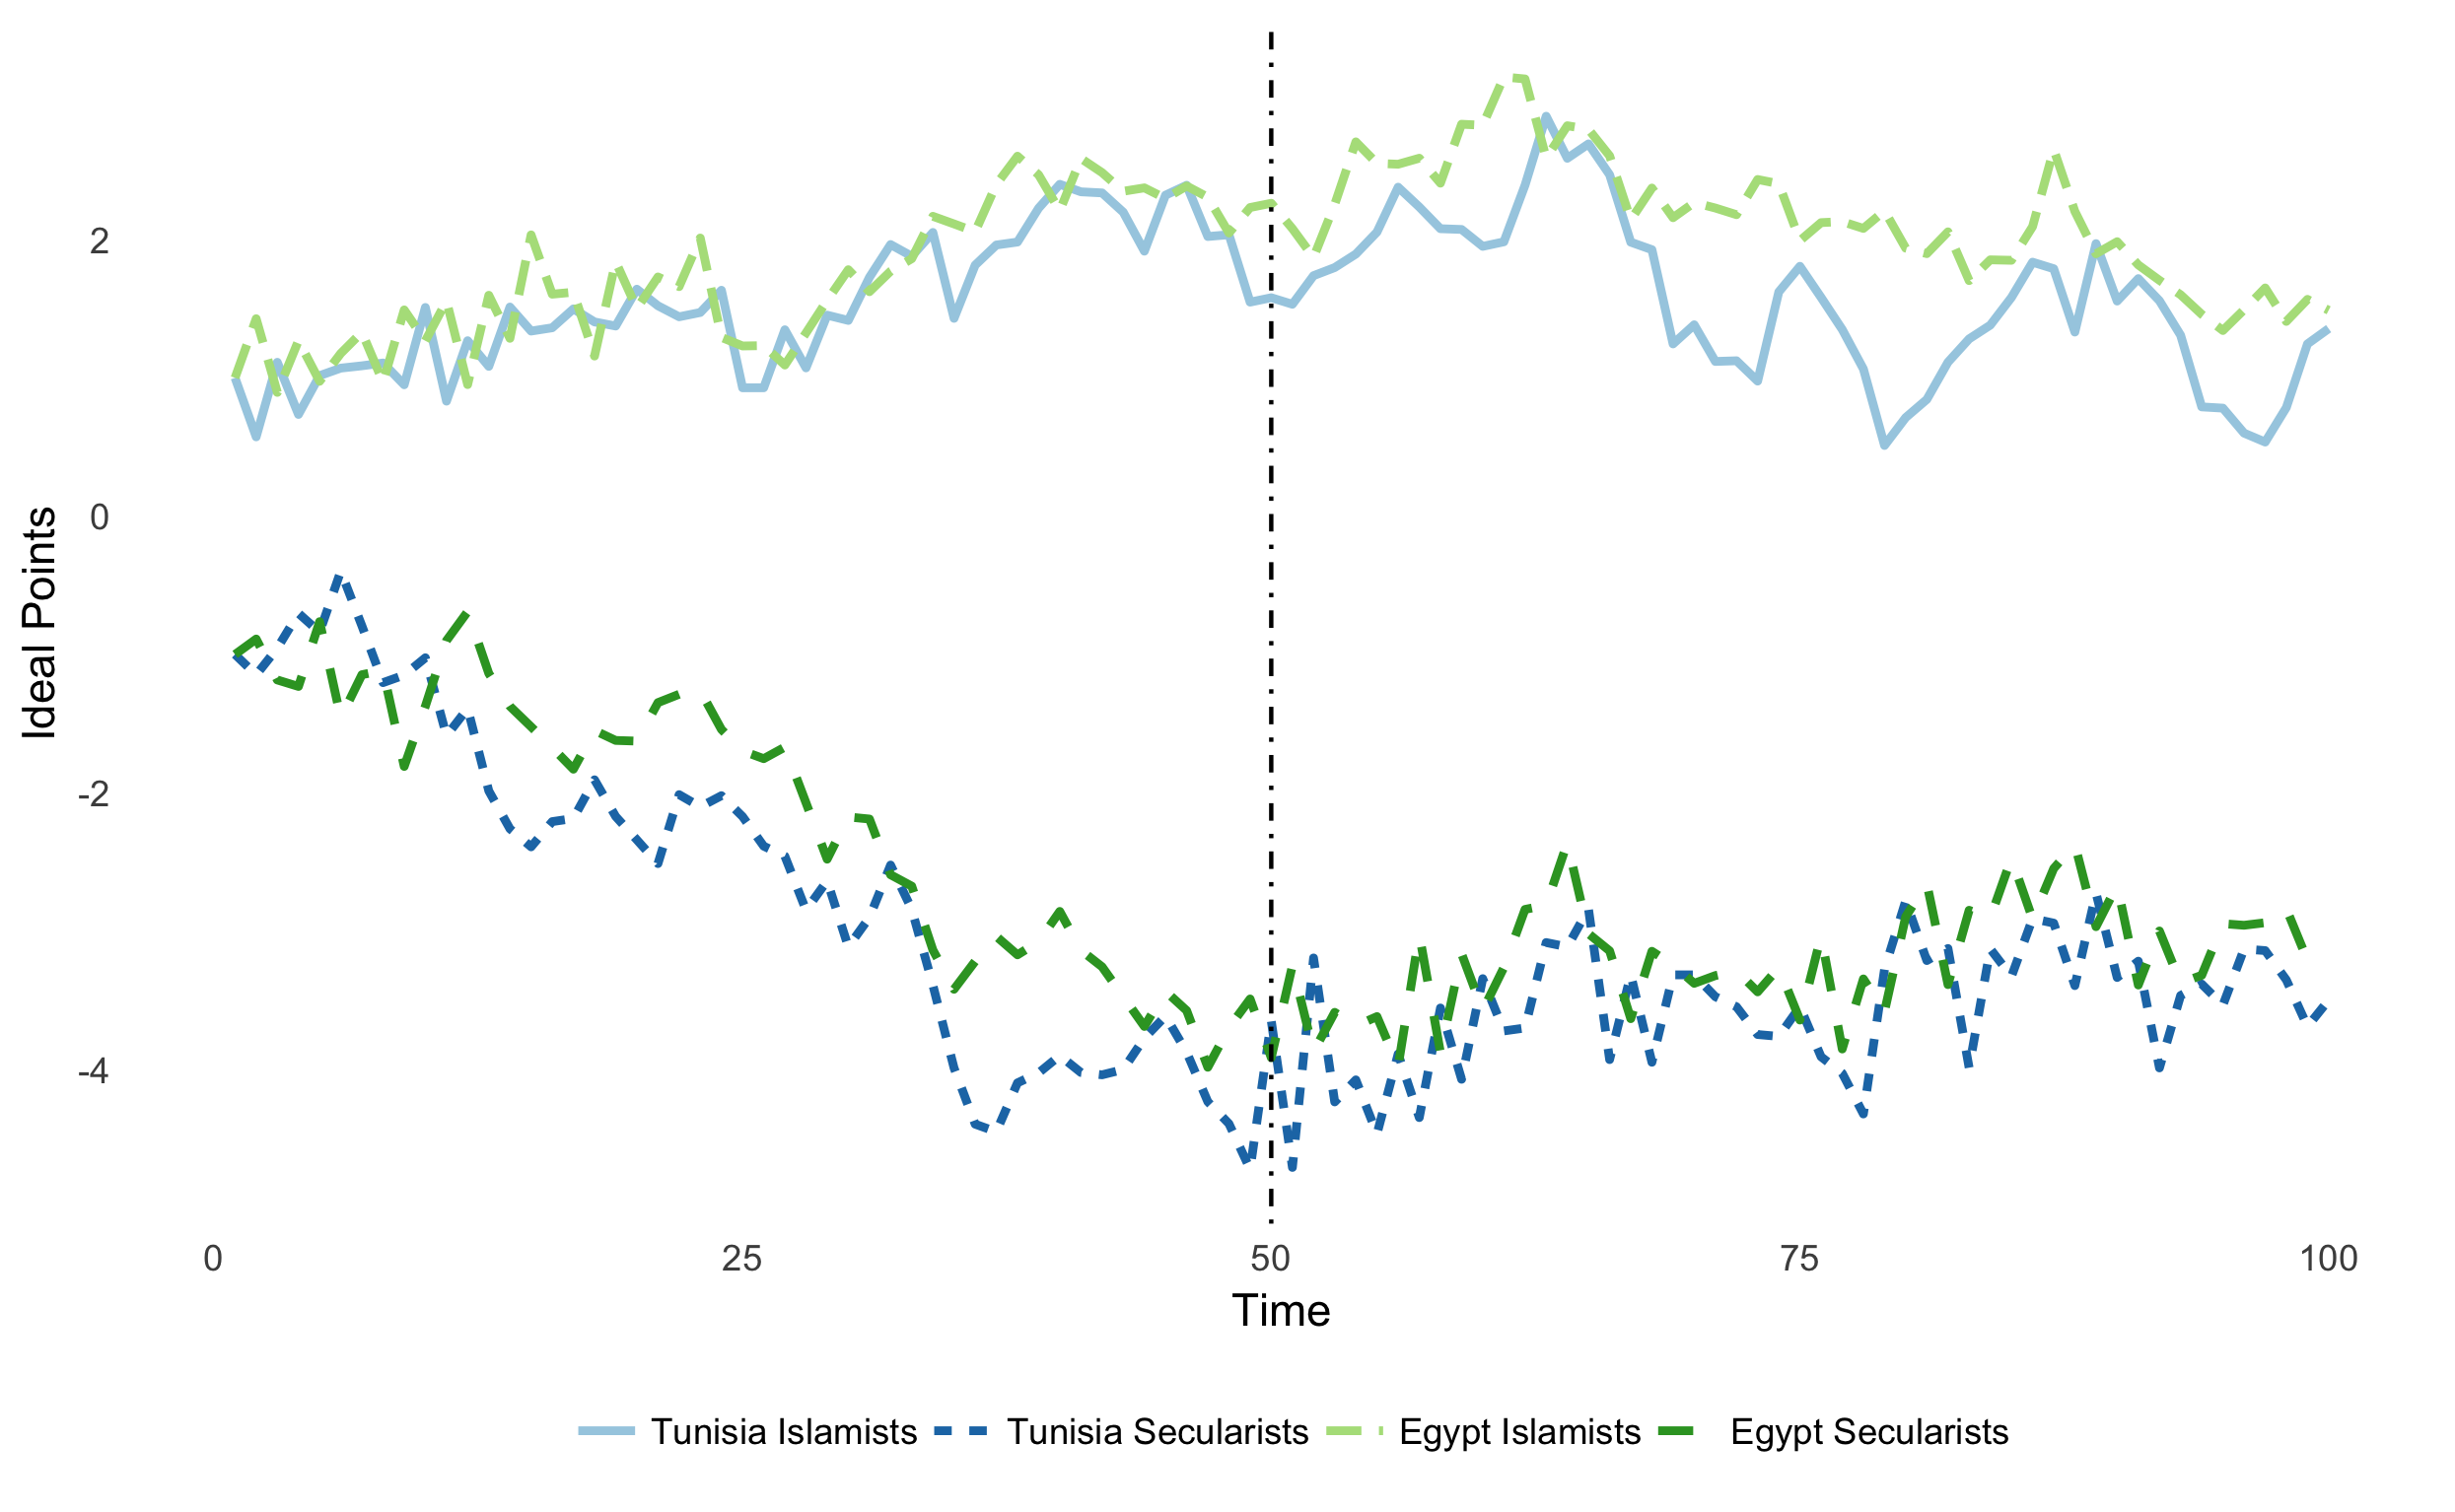
\includegraphics[width=.9\linewidth]{ecm_example.png}
 \end{figure}

The vertical line in Figure \ref{sim_data} shows a point where we changed the values for the $\gamma$ parameter governing the level of co-integration. For the top time series, $\gamma$ fell, so after the dotted line the two time series do not track each other as closely. For the bottom time series, $\gamma$ increased, causing the two time series to follow each other more closely. For this reason, the $\gamma$ parameter is one way to test the hypotheses by examining whether $\gamma$ varies before and after Morsi's coup. We can also allow the co-integrating vector to vary so that the extent of feedback across countries changes pre and post-coup. However, we are limited in being able to only estimate a single value for these summary statistics, so it may be difficult to interpret them as cleanly as in Figure \ref*{true_pars} given that the effect of the polarizing event may not last longer than a few time periods. In addition to summary statistics, we can also examine the time series for cross-national shocks before and after the coup so that we can measure the extent to which shocks from one time series impact ideological estimates in another country, which is known as an impulse-response function (IRF).
\begin{figure}[!h]
	\caption{Recovery of True Parameter Values}\label{true_pars}
	\centering
	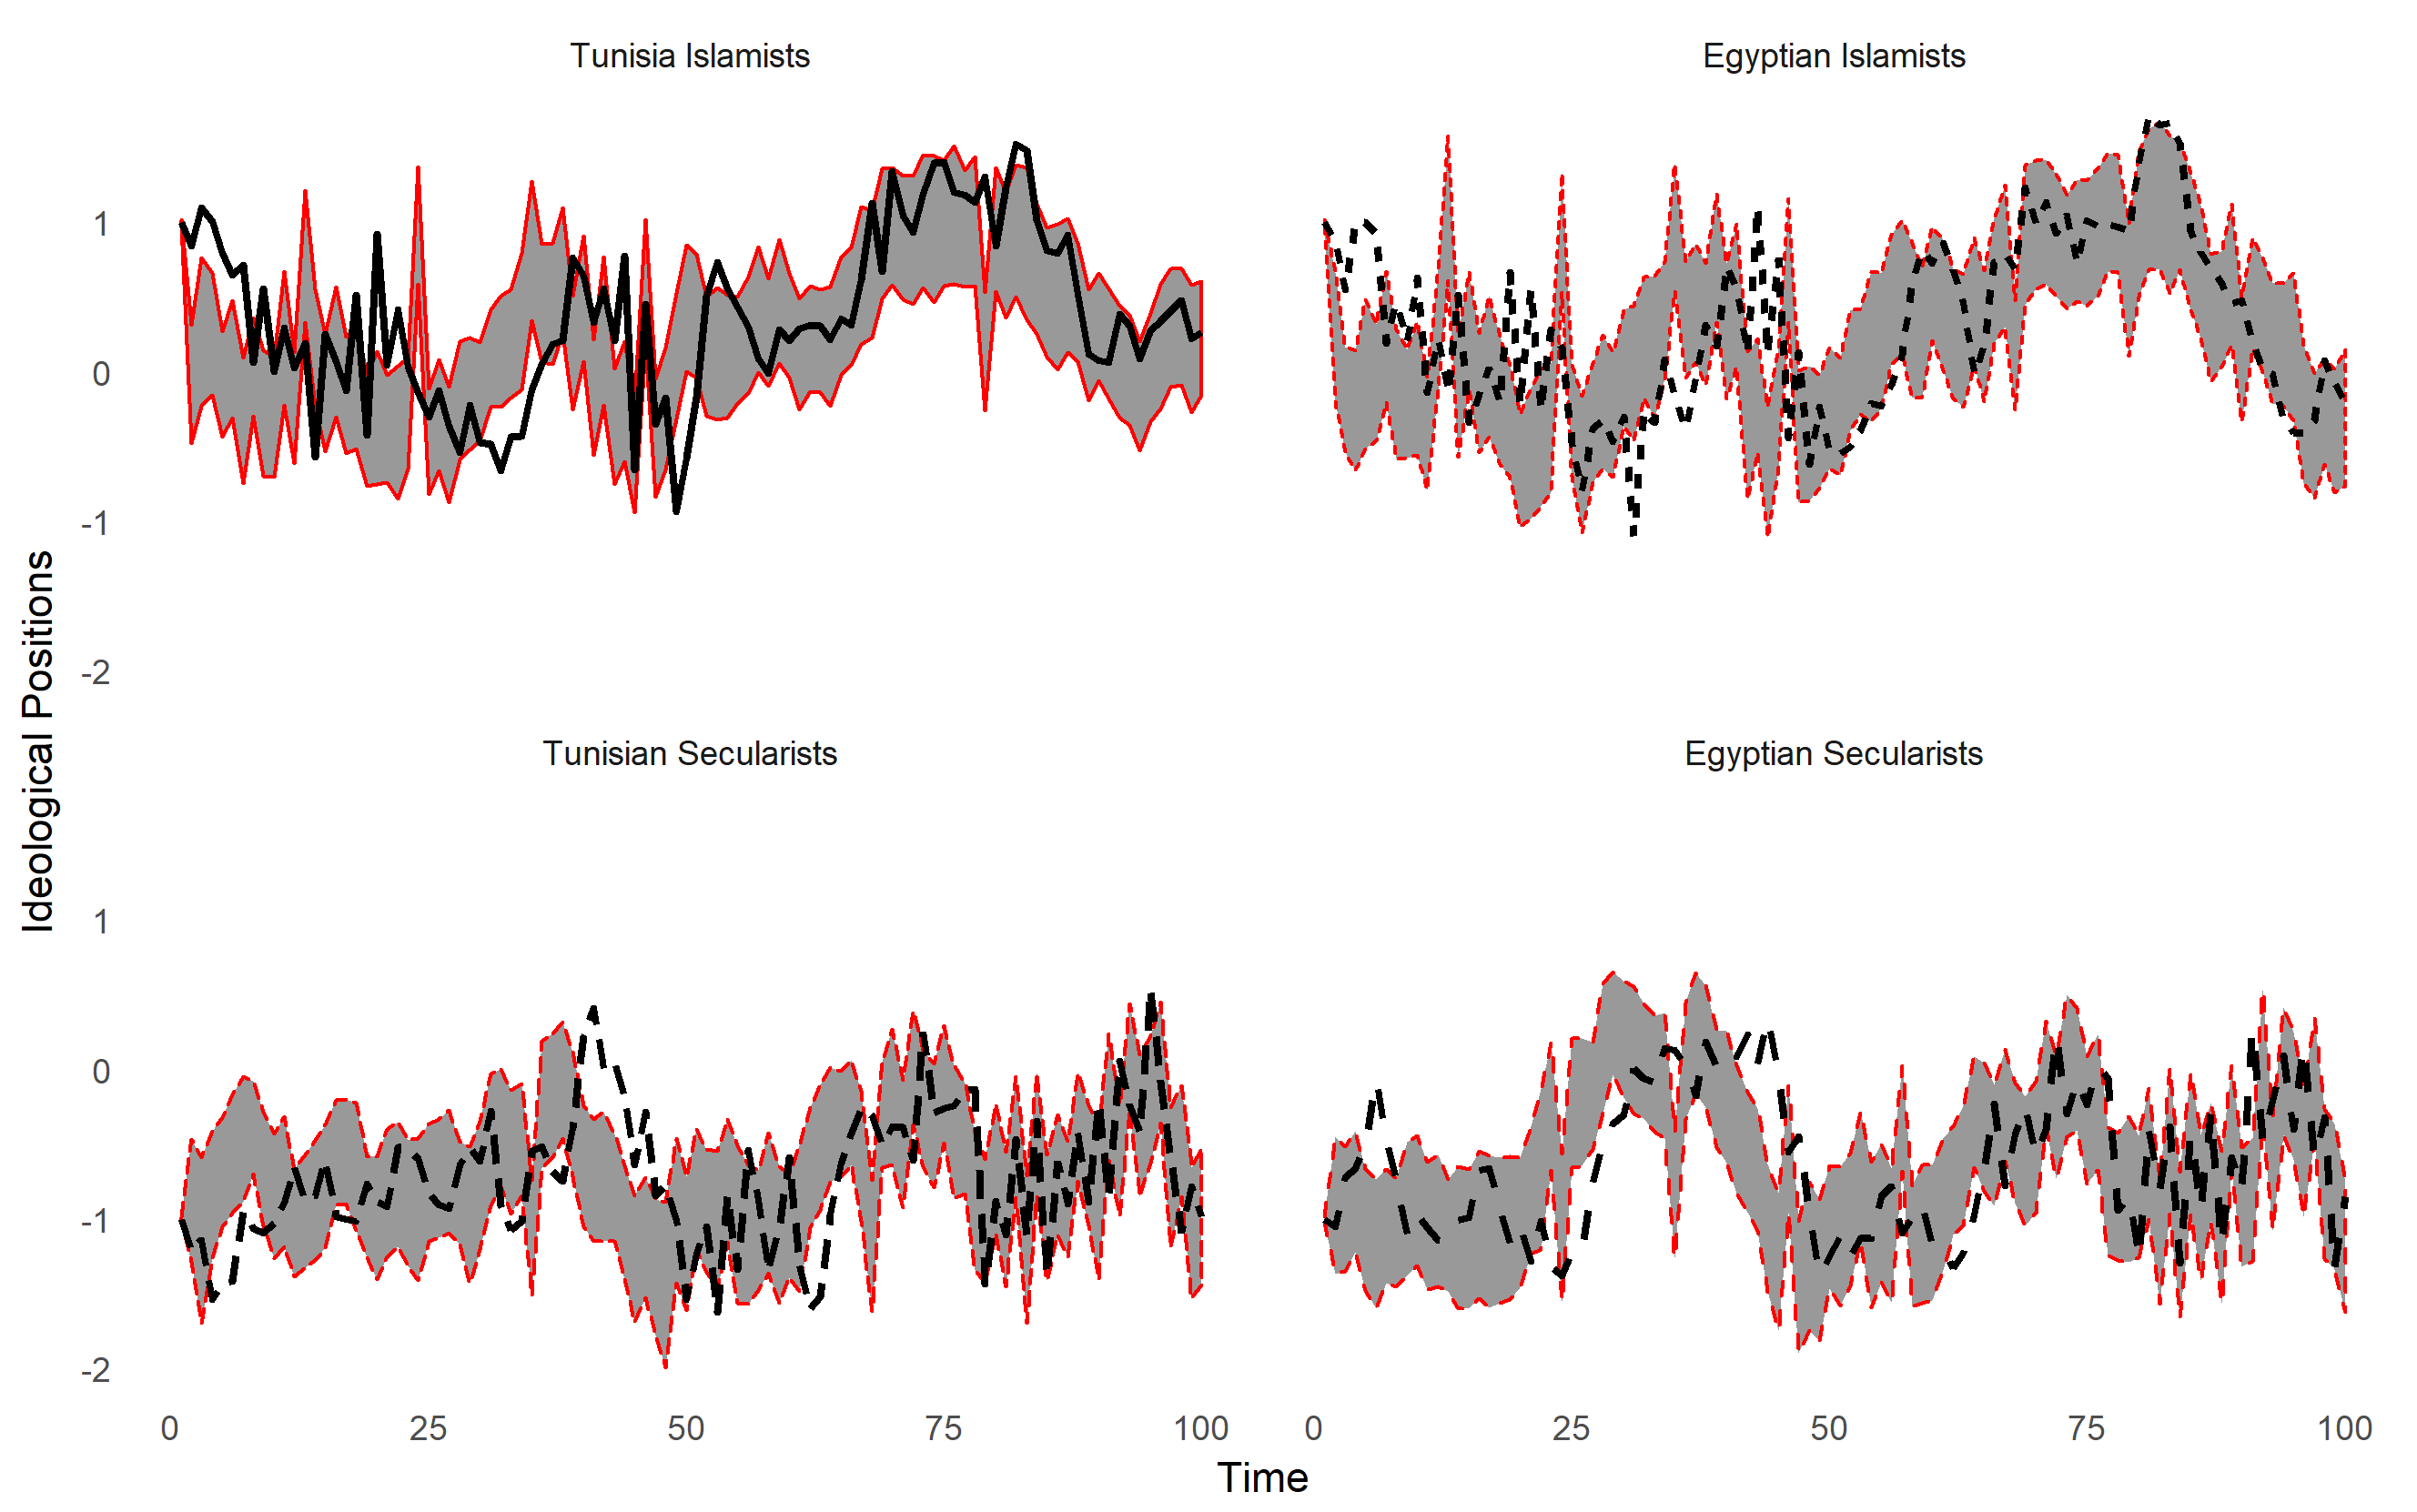
\includegraphics[width=.9\linewidth]{true_estimated.png}
\end{figure}

Finally, Figure \ref{true_pars} shows the performance of the model at recovering the latent time series using Bayesian MCMC estimation within the Stan framework \parencite{carpenter2017}. While the recovery is not perfect, it is able to follow the same path of the generated data. The uncertainty around the latent process will by necessity be larger because the time series themselves are unobserved.

\section*{Model Results}

We present here results from MCMC estimation with four independent chains to test for convergence. All of the estimated values achieved Rhat values below 1.1, a strong sign of convergence of the chains to a stationary distribution \parencite{gelman1992}. The final estimation produced 18,123 each of discrimination and intercept parameters for all of the citizens in the model, but we will focus on the four group parameters that varied over time, one for each country-ideological pairing: Tunisian secularists, Egyptian secularists, Tunisian Islamists, and Tunisian secularists.

We first present a plot showing the estimated ideal points for the four ideological groups along with a vertical line showing when the military coup against Mohammed Morsi occurred. The confidence intervals on the chart reflects the 10\%-90\% density region of the posterior, hereafter referred to as the high-posterior density (HPD) interval. The HPD intervals are much smaller for the secularists because there are more Twitter accounts in the sample for these groups. As can be seen, the ideal points for Islamists exhibit substantial movement over time, and prior to the coup the two time series were tracking each other very closely. Immediately after the coup, both Islamists and secularists in Egypt show a large shock to their ideal points. Within the space of a week, Egyptian Islamists moved a distance equivalent to four standard deviations along the ideal point scale from 1 to -1. This finding provides initial support for hypotheses 1 and 2 regarding our prior belief that polarizing events would have a large and significant effect on latent ideological scores. The immediate impact, though, of the coup on ideological groups in Tunisia is relatively modest and less than we would have expected from a purely visual inspection.
 \begin{figure}[!h]
 	\centering
	\caption{Estimated Ideal Point Locations for Cross-National Ideological Groups}\label{arab_id_facet}
	\centering
	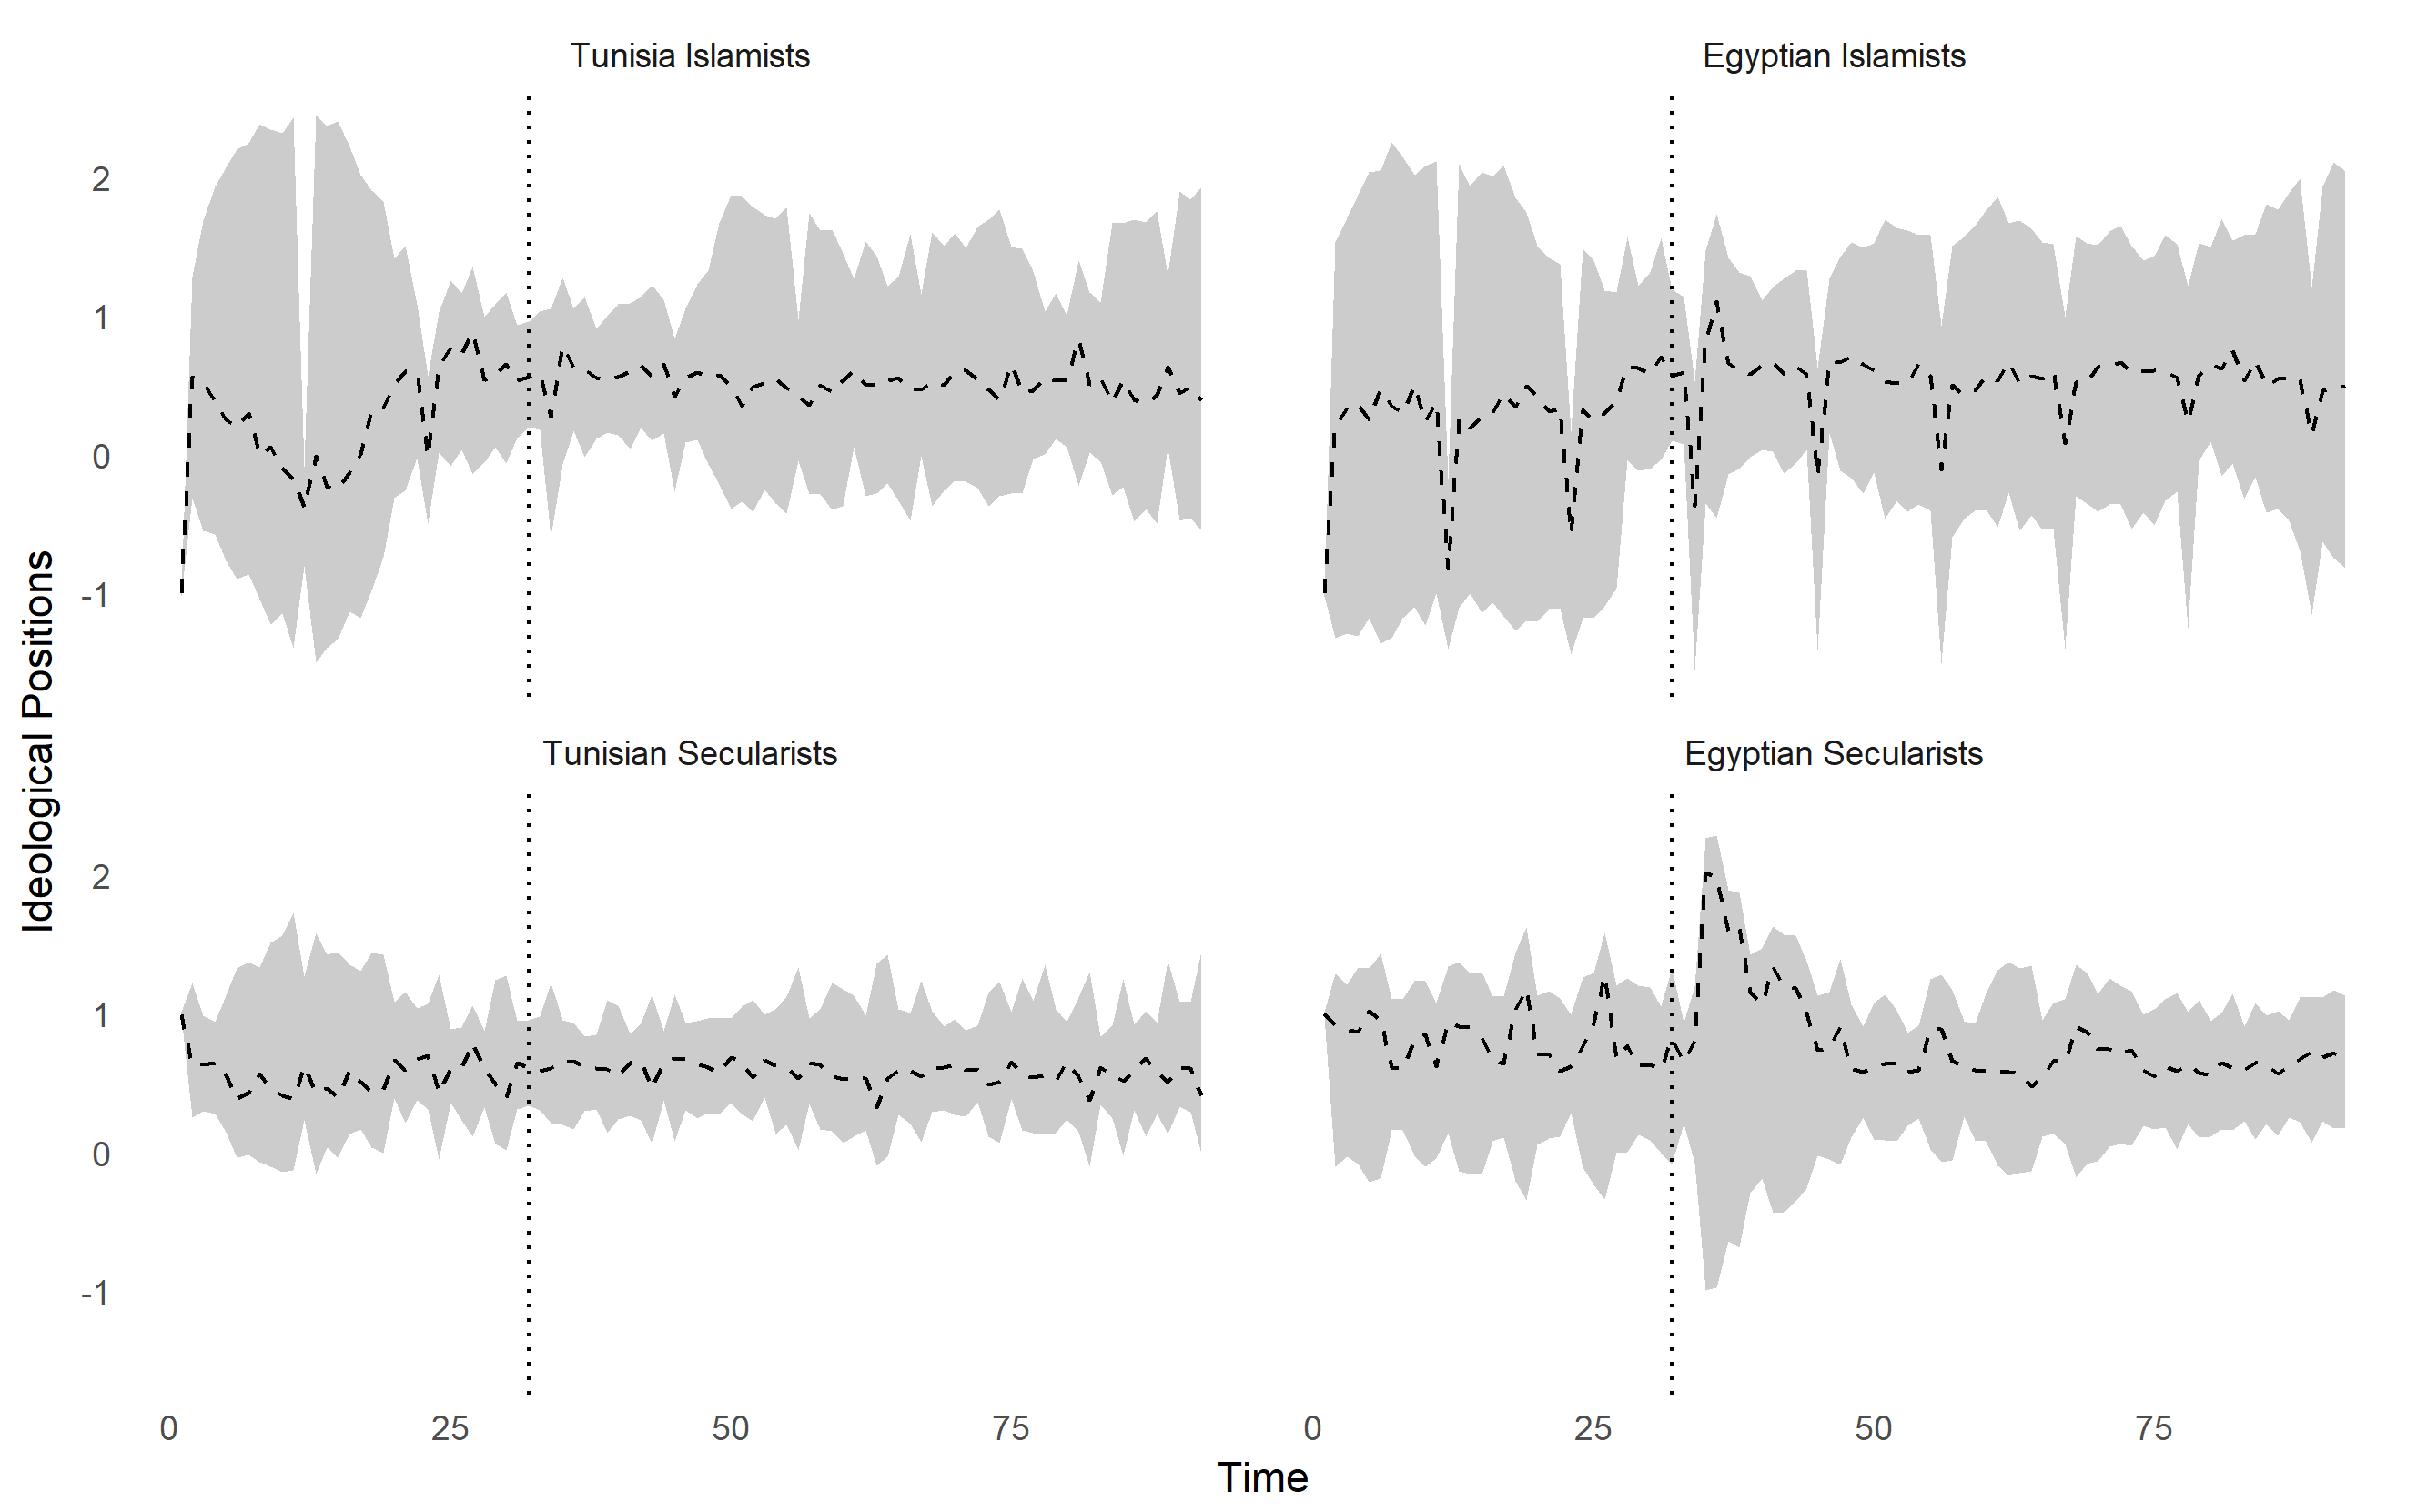
\includegraphics[width=.9\linewidth]{arab_ideology}
\end{figure}

While we can clearly see the shock, it is not so easy to see all trends in the series visually. To see the relationships better, we show these trend lines without HPD intervals and overlapping country/ideological groups in Figures \ref{arab_id_facet} and \ref{country_facet}. While it can be difficult to spot patterns in time series with the naked eye, it is very clear that Islamists track with each other much more than secularists do in general, although by the end of the series secularists were beginning to move much closer in the ideal point space. 
 \begin{figure}[!h]
 	\centering
	\caption{Estimated Ideal Point Locations by Religion}\label{religion_facet}
	\centering
	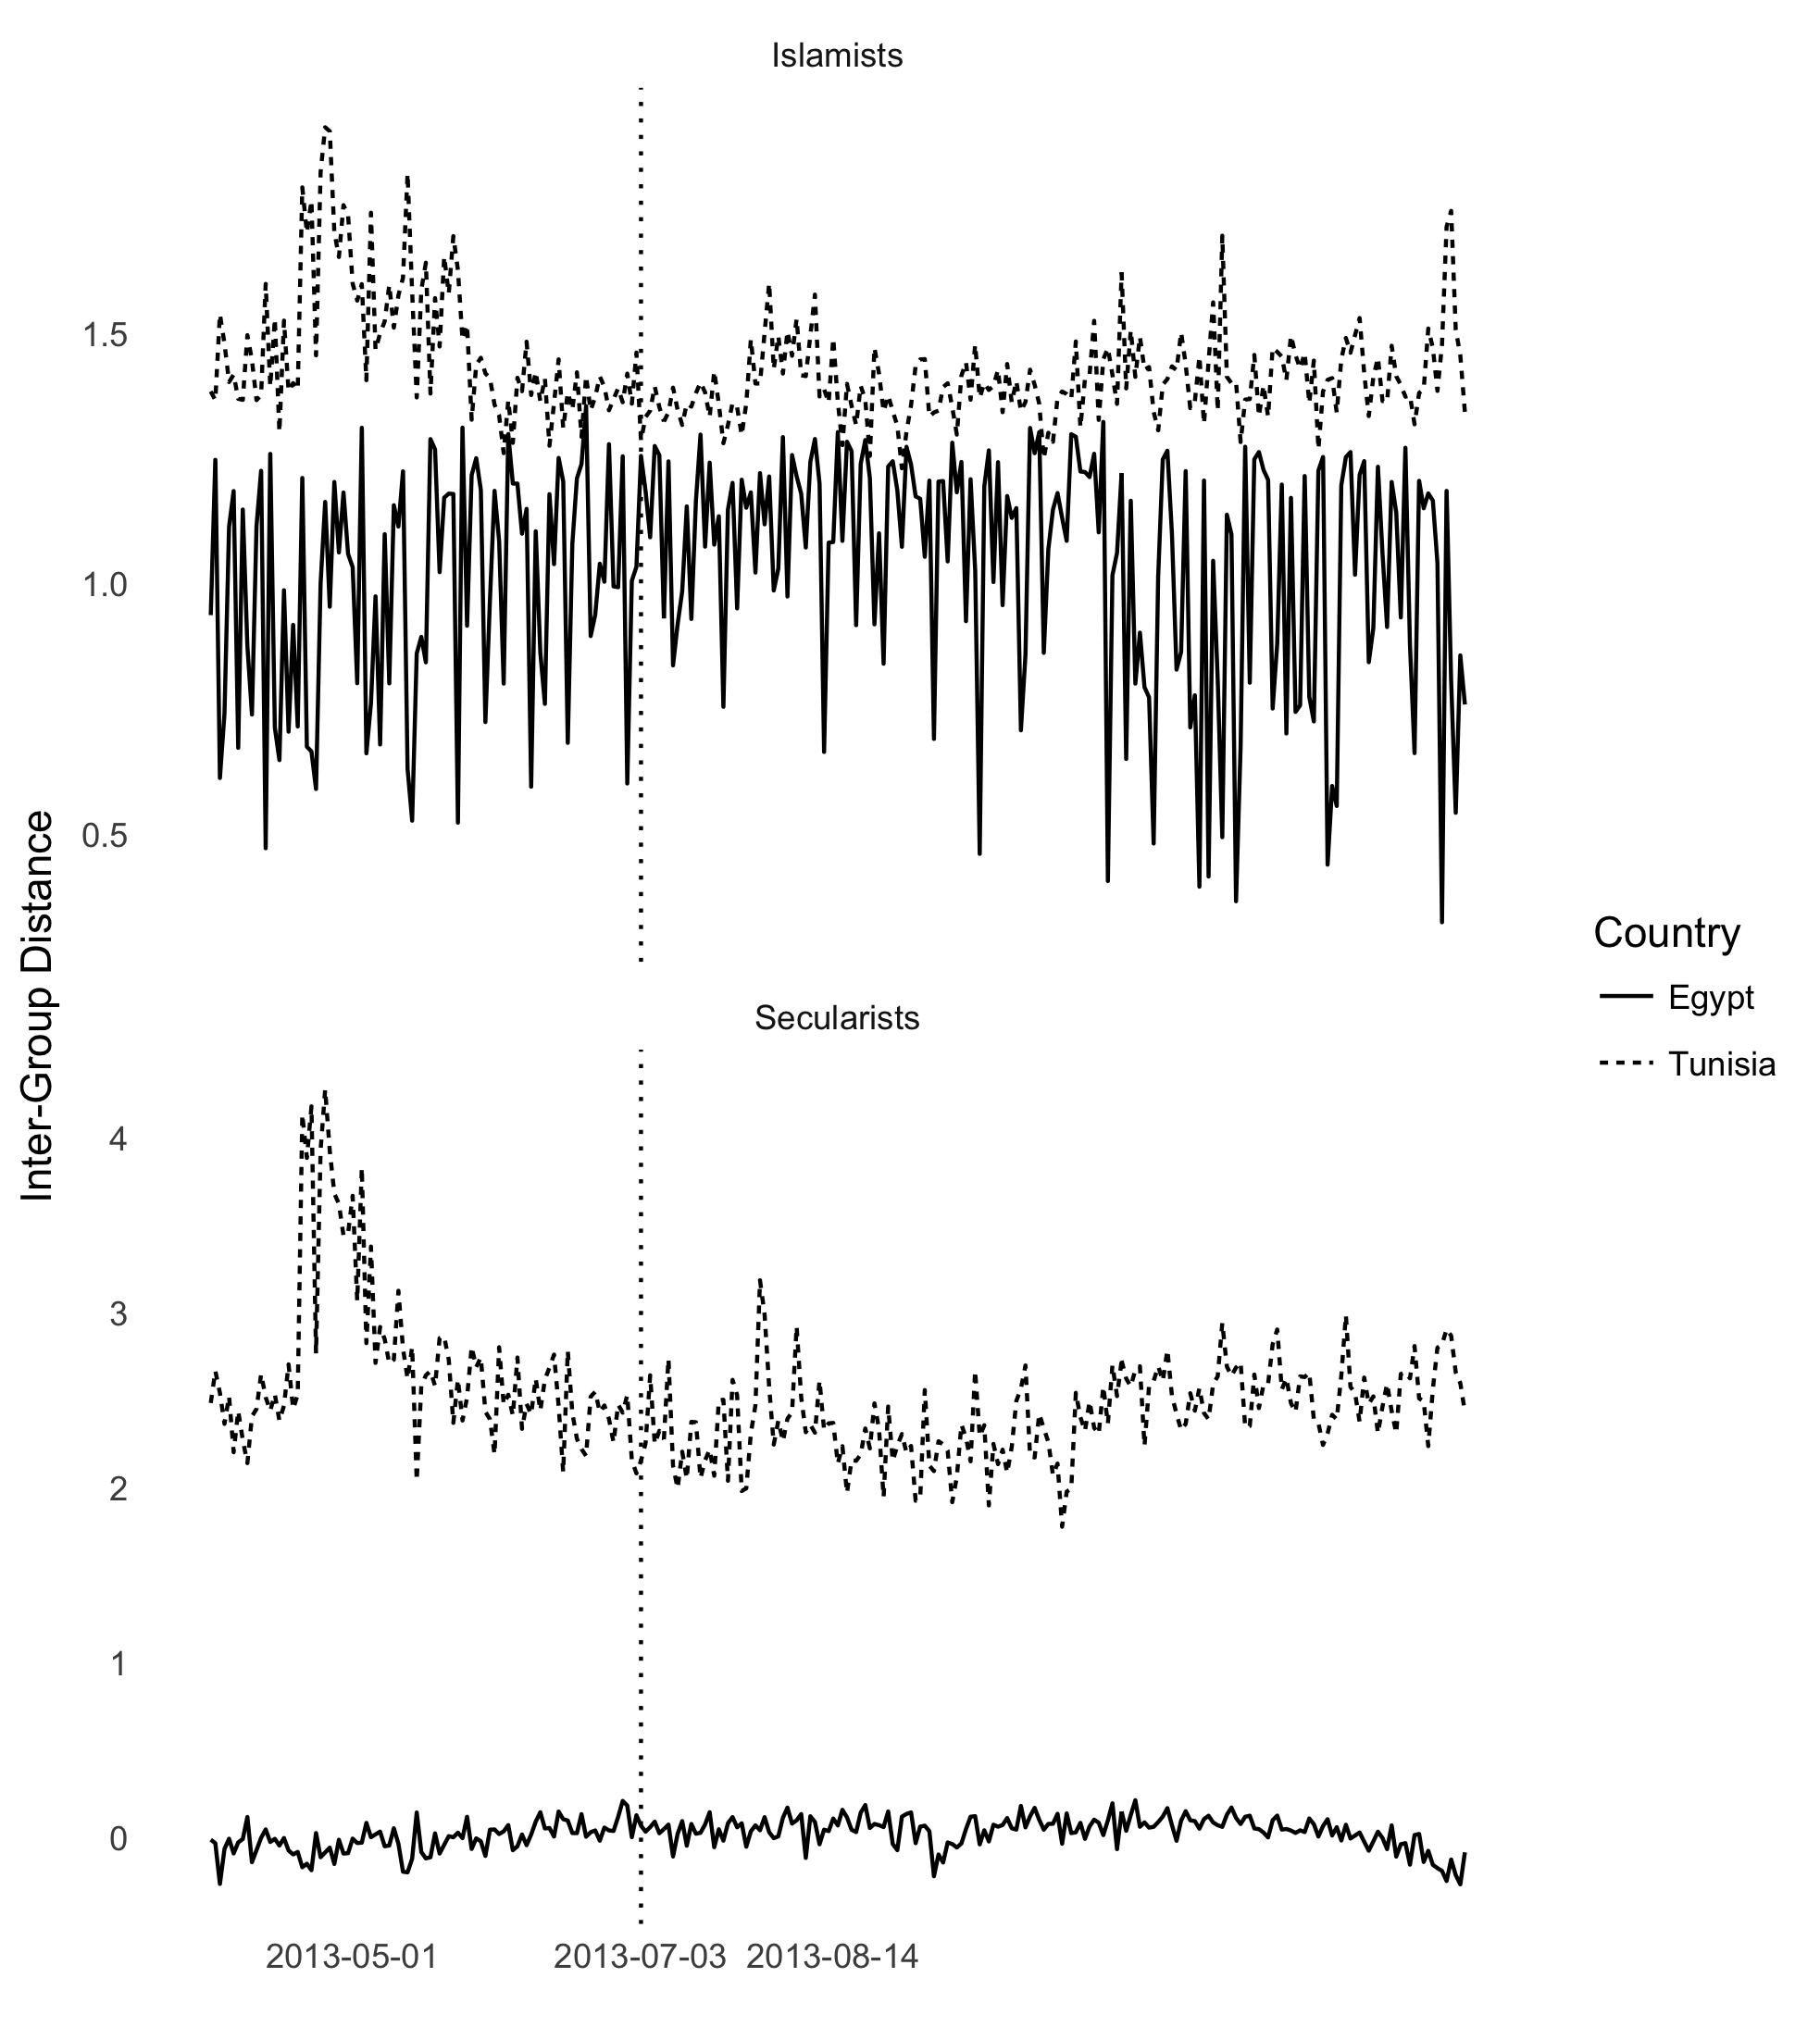
\includegraphics[width=.9\linewidth]{religion_coint}
\end{figure}
 \begin{figure}[!h]
 	\centering
	\caption{Estimated Ideal Point Locations by Country}\label{country_facet}
	\centering
	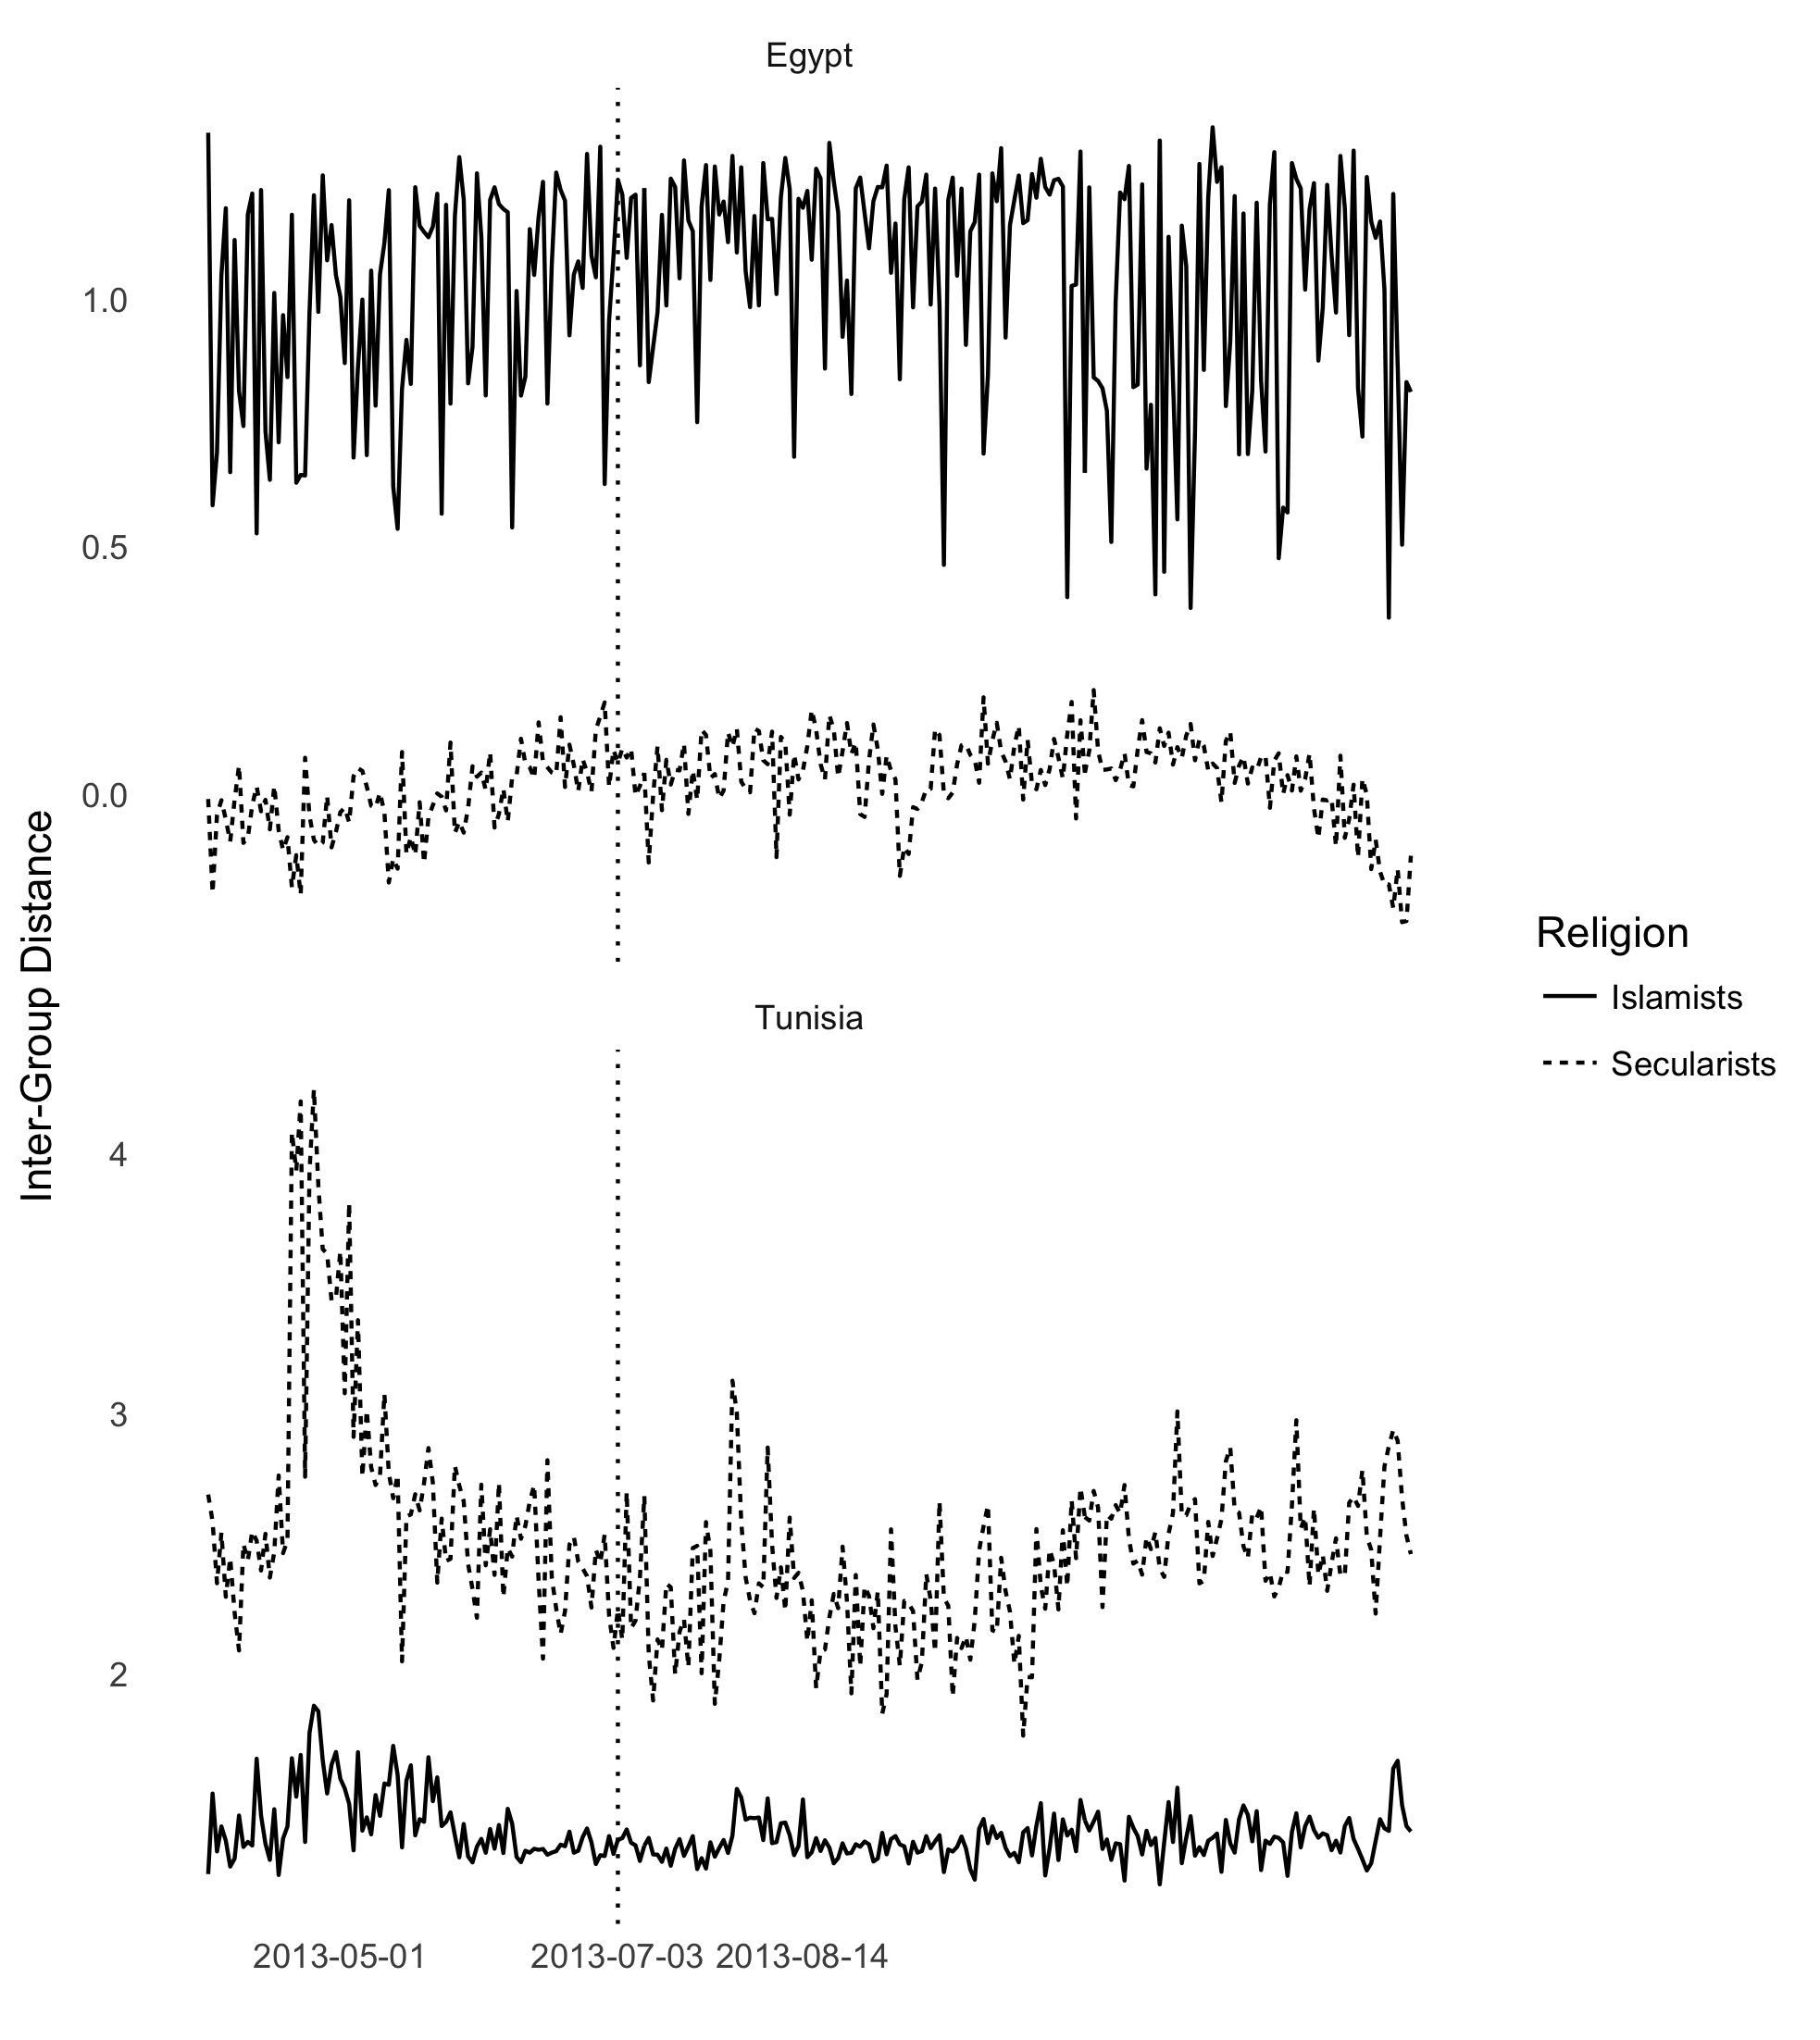
\includegraphics[width=.9\linewidth]{country_coint}
\end{figure}

What is clear from Figure \ref{country_facet} is that ideal points in Egypt exhibit wider polarization in general than secularists and Islamists in Tunisia. In Egypt, Islamists and secularists are far apart prior to the coup, and after the period of instability following the coup, they diverge again, although there is some reconciliation by the end of the time series. By comparison, ideological groups in Tunisia tend to stay closer, which is a sign that users will tend to retweet a more diverse ideological group of elites. 

We can look at the $\gamma_g$ parameters to see how well we can quantify the role of co-integration in the time series. The $\gamma_g$ shown in Figure \ref{gamma_joy} and \ref{gamma_diff} reveal that pre-coup, Islamist were estimated to have a higher level of co-integration, but that the estimate is very imprecise. Post-coup, the estimate is much more precise and still higher than the secularists, although on average it is lower than pre-coup. Secularists exhibited less movement in their $\gamma_g$ parameter, although it increases modestly after the coup. Given the imprecision in the estimate for the Islamists prior to the coup, the best that we can say from inspection of these parameters is that the model is able to confirm that Islamists do track each other more closely than secularists during this time period.
 \begin{figure}[!h]
	\centering
	\caption{Estimated Pre and Post-Coup $\gamma_g$}\label{gamma_joy}
	\centering
	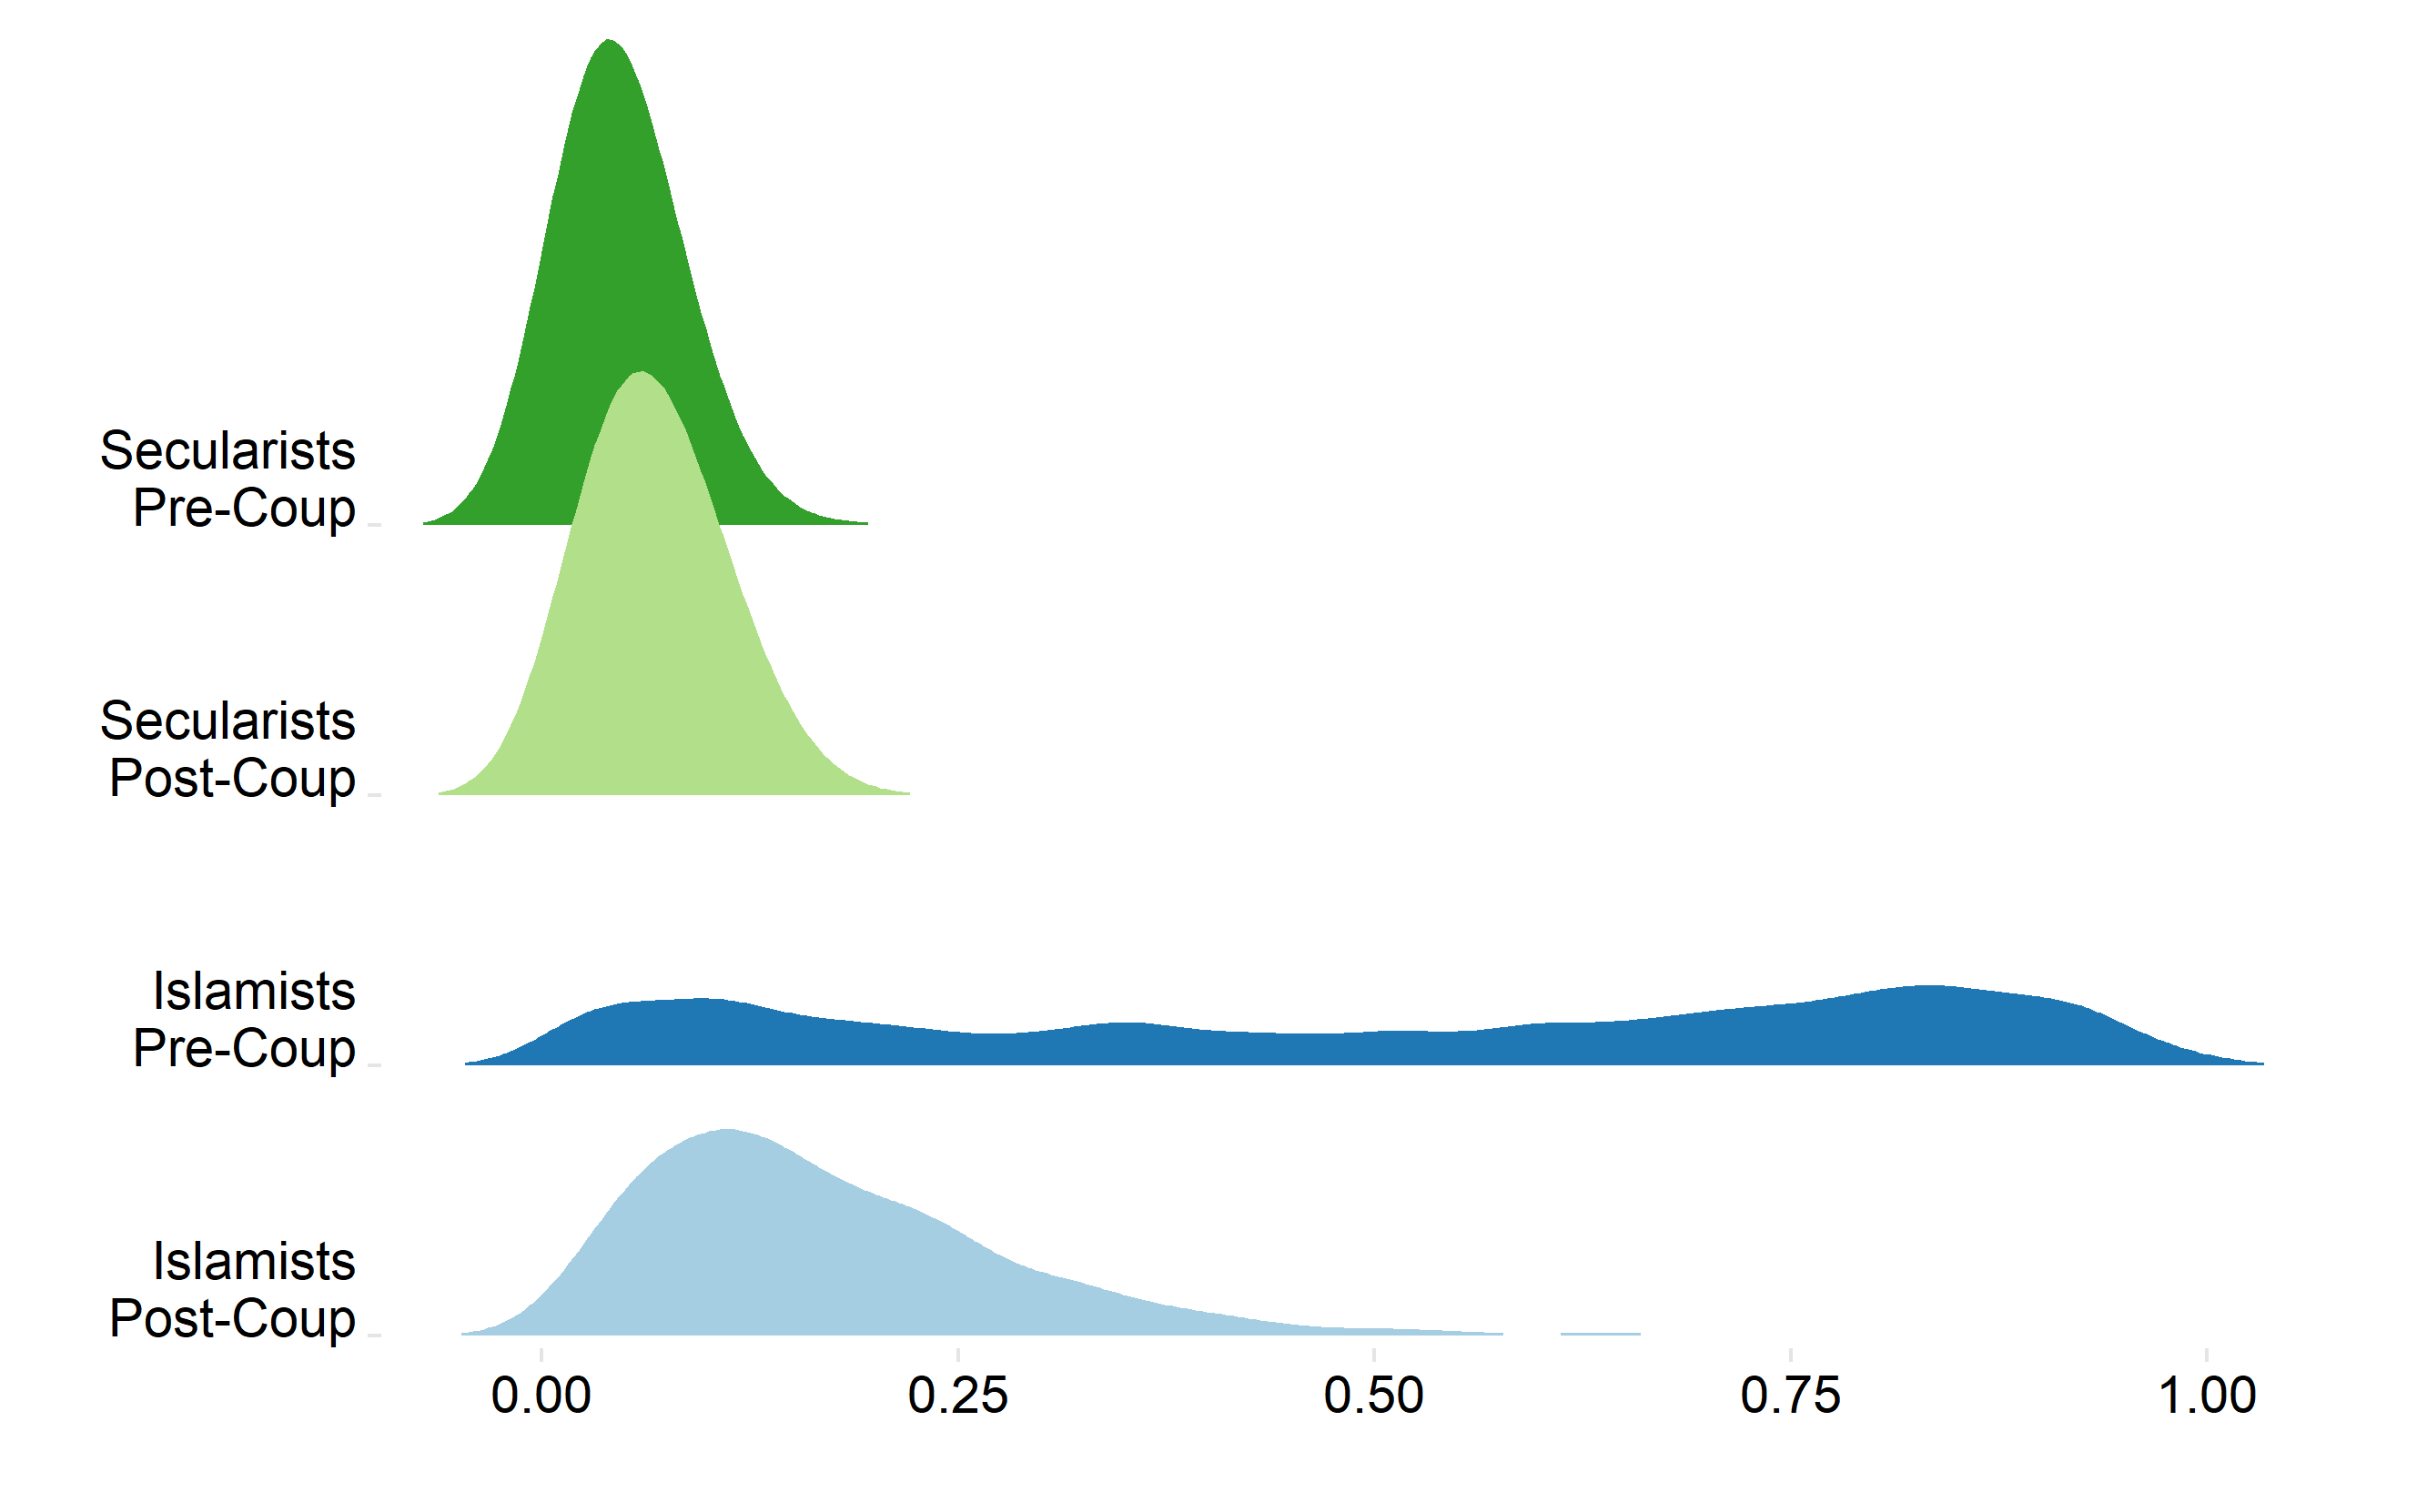
\includegraphics[width=.9\linewidth]{gamma_joy}
\end{figure}
\begin{figure}[!h]
	\centering
	\caption{Difference in Pre vs. Post-Coup $\gamma_g$}\label{gamma_diff}
	\centering
	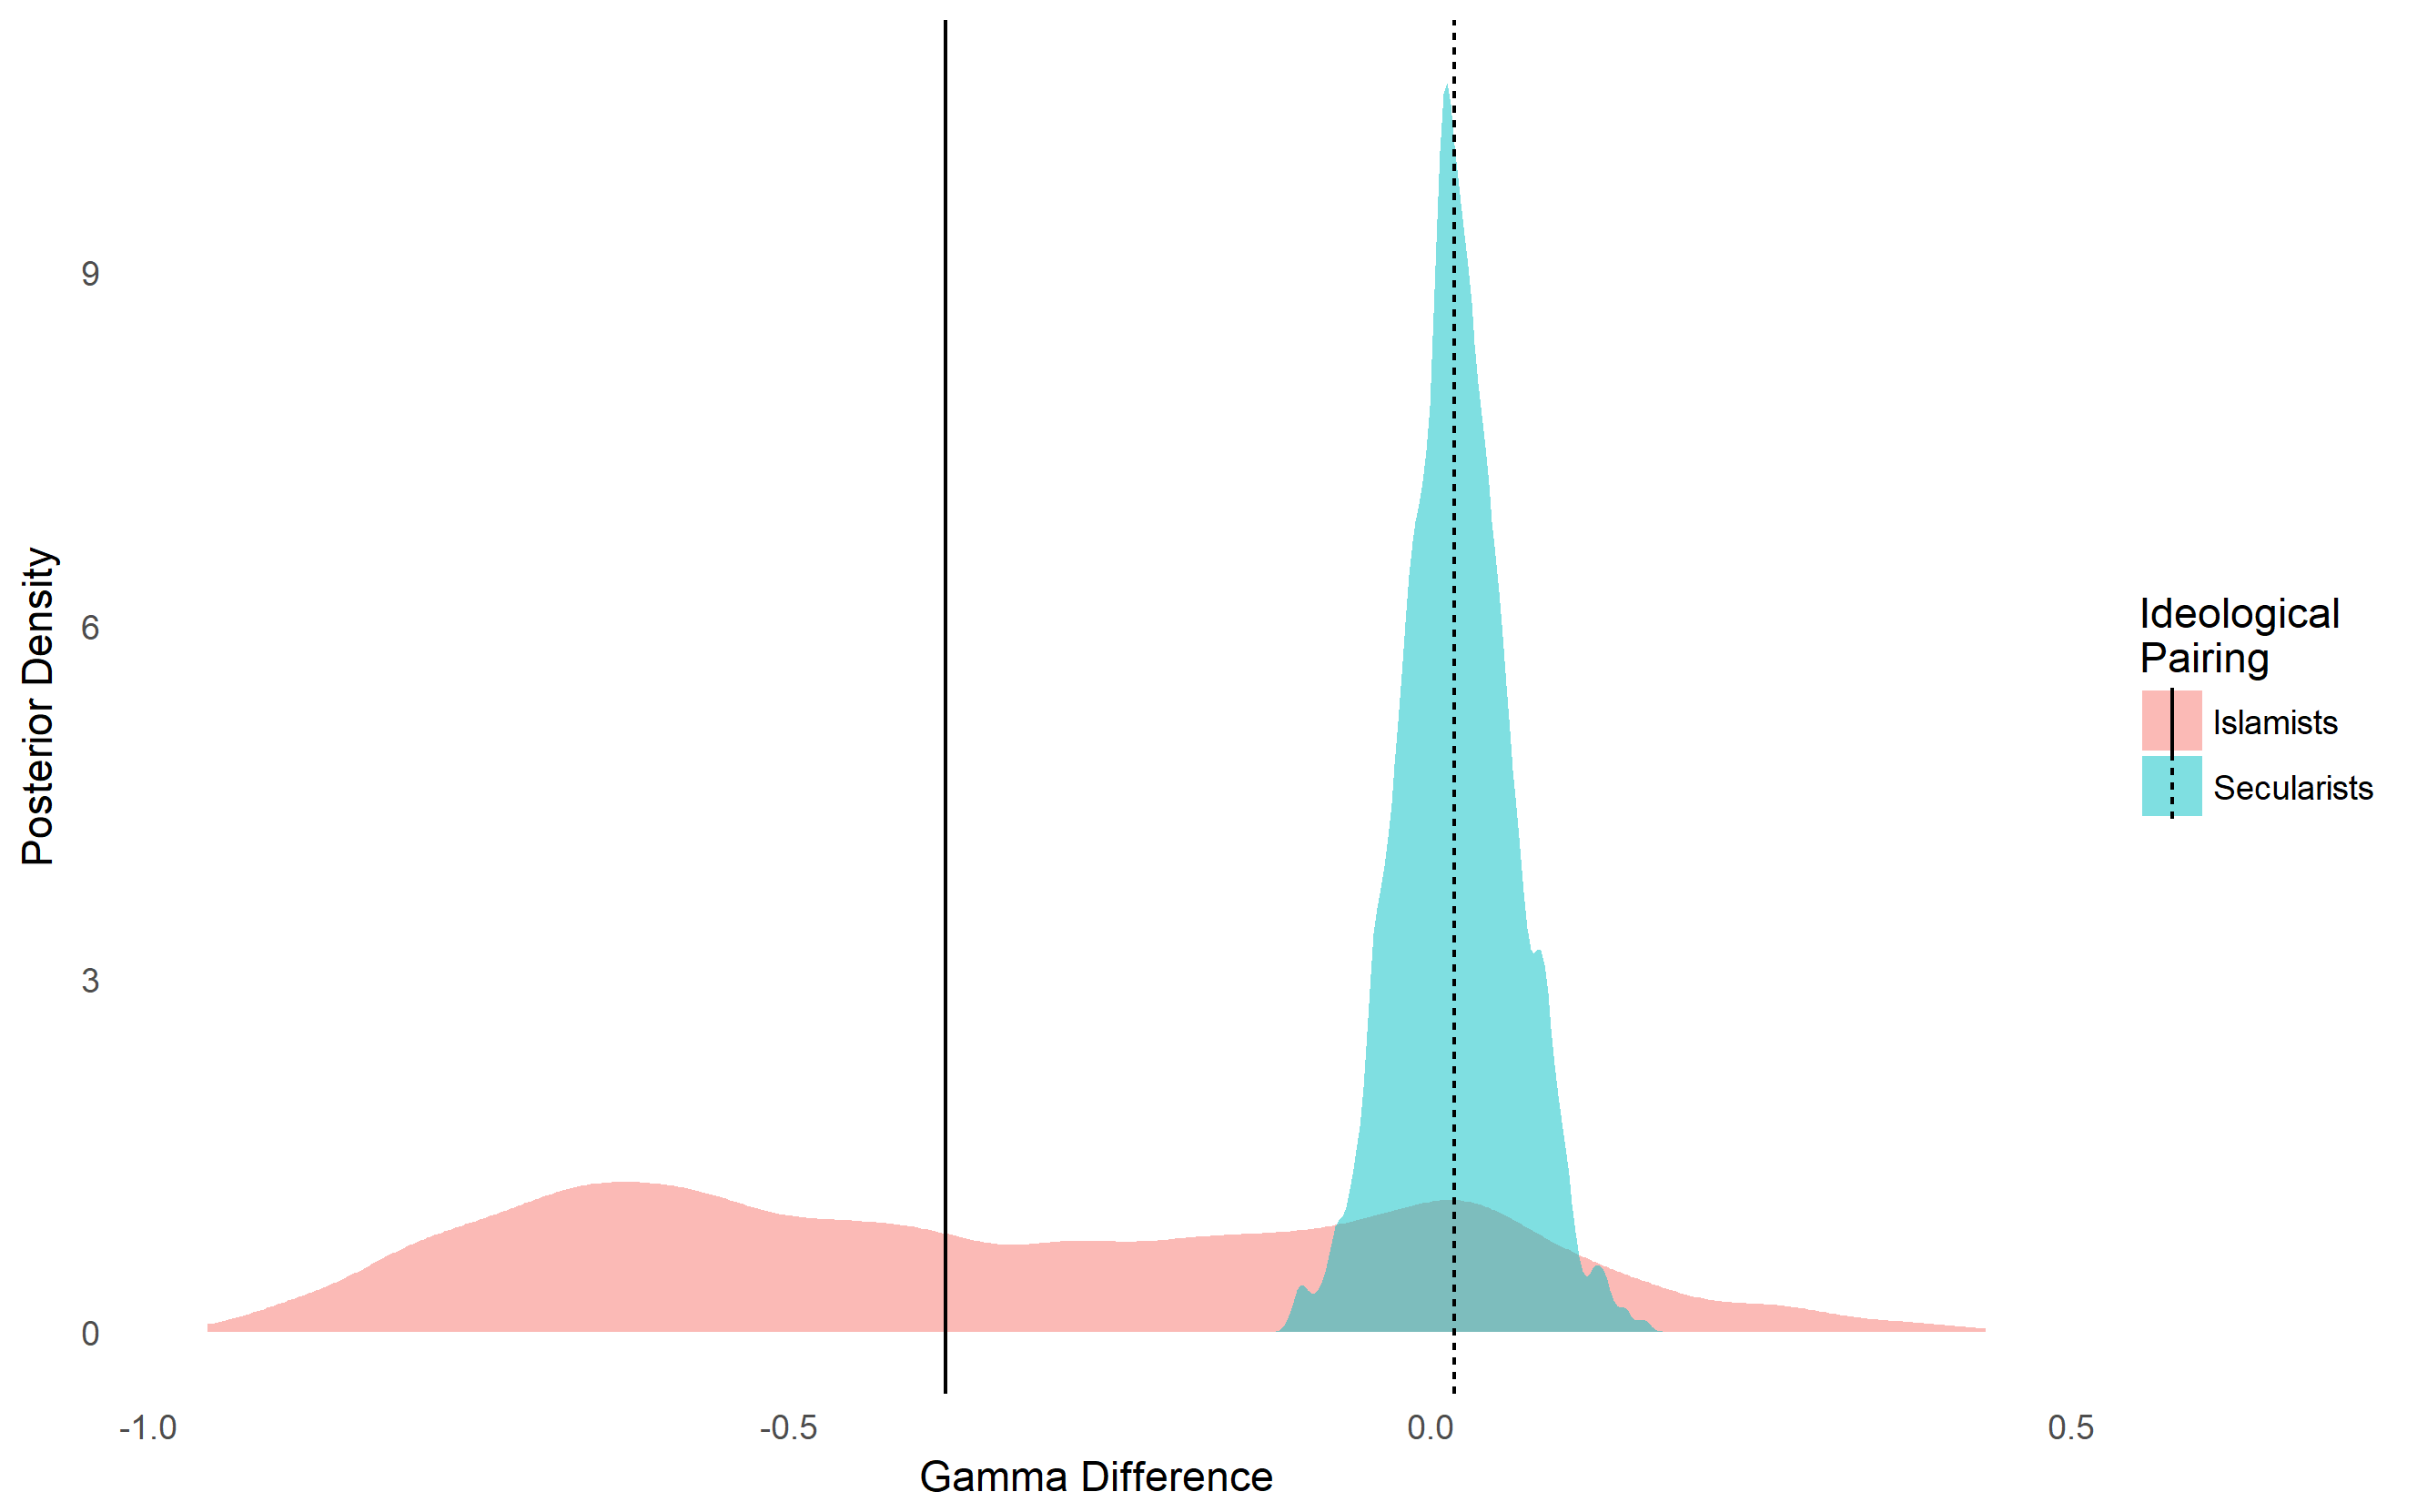
\includegraphics[width=.9\linewidth]{gamma_diff}
\end{figure}


In addition to the $\gamma_g$ parameters that measure the overall level of co-integration in the system, we can look more specifically at the co-integrating vector that determines in what direction feedback happens. Figure \ref{adj} shows the co-integration vector for both groups in a model that allows the co-integration vector to vary before and after the coup. A value of one for this parameter indicates that both time series tend to influence each other equally. This figure shows that the coup did not noticeably affect the overall direction of feedback in the system in either a positive or negative direction. After the coup, both groups tended to influence each other in roughly the same amount.
 \begin{figure}[!h]
	\centering
	\caption{Estimated Pre and Post-Coup Co-integrating Vectors}\label{adj}
	\centering
	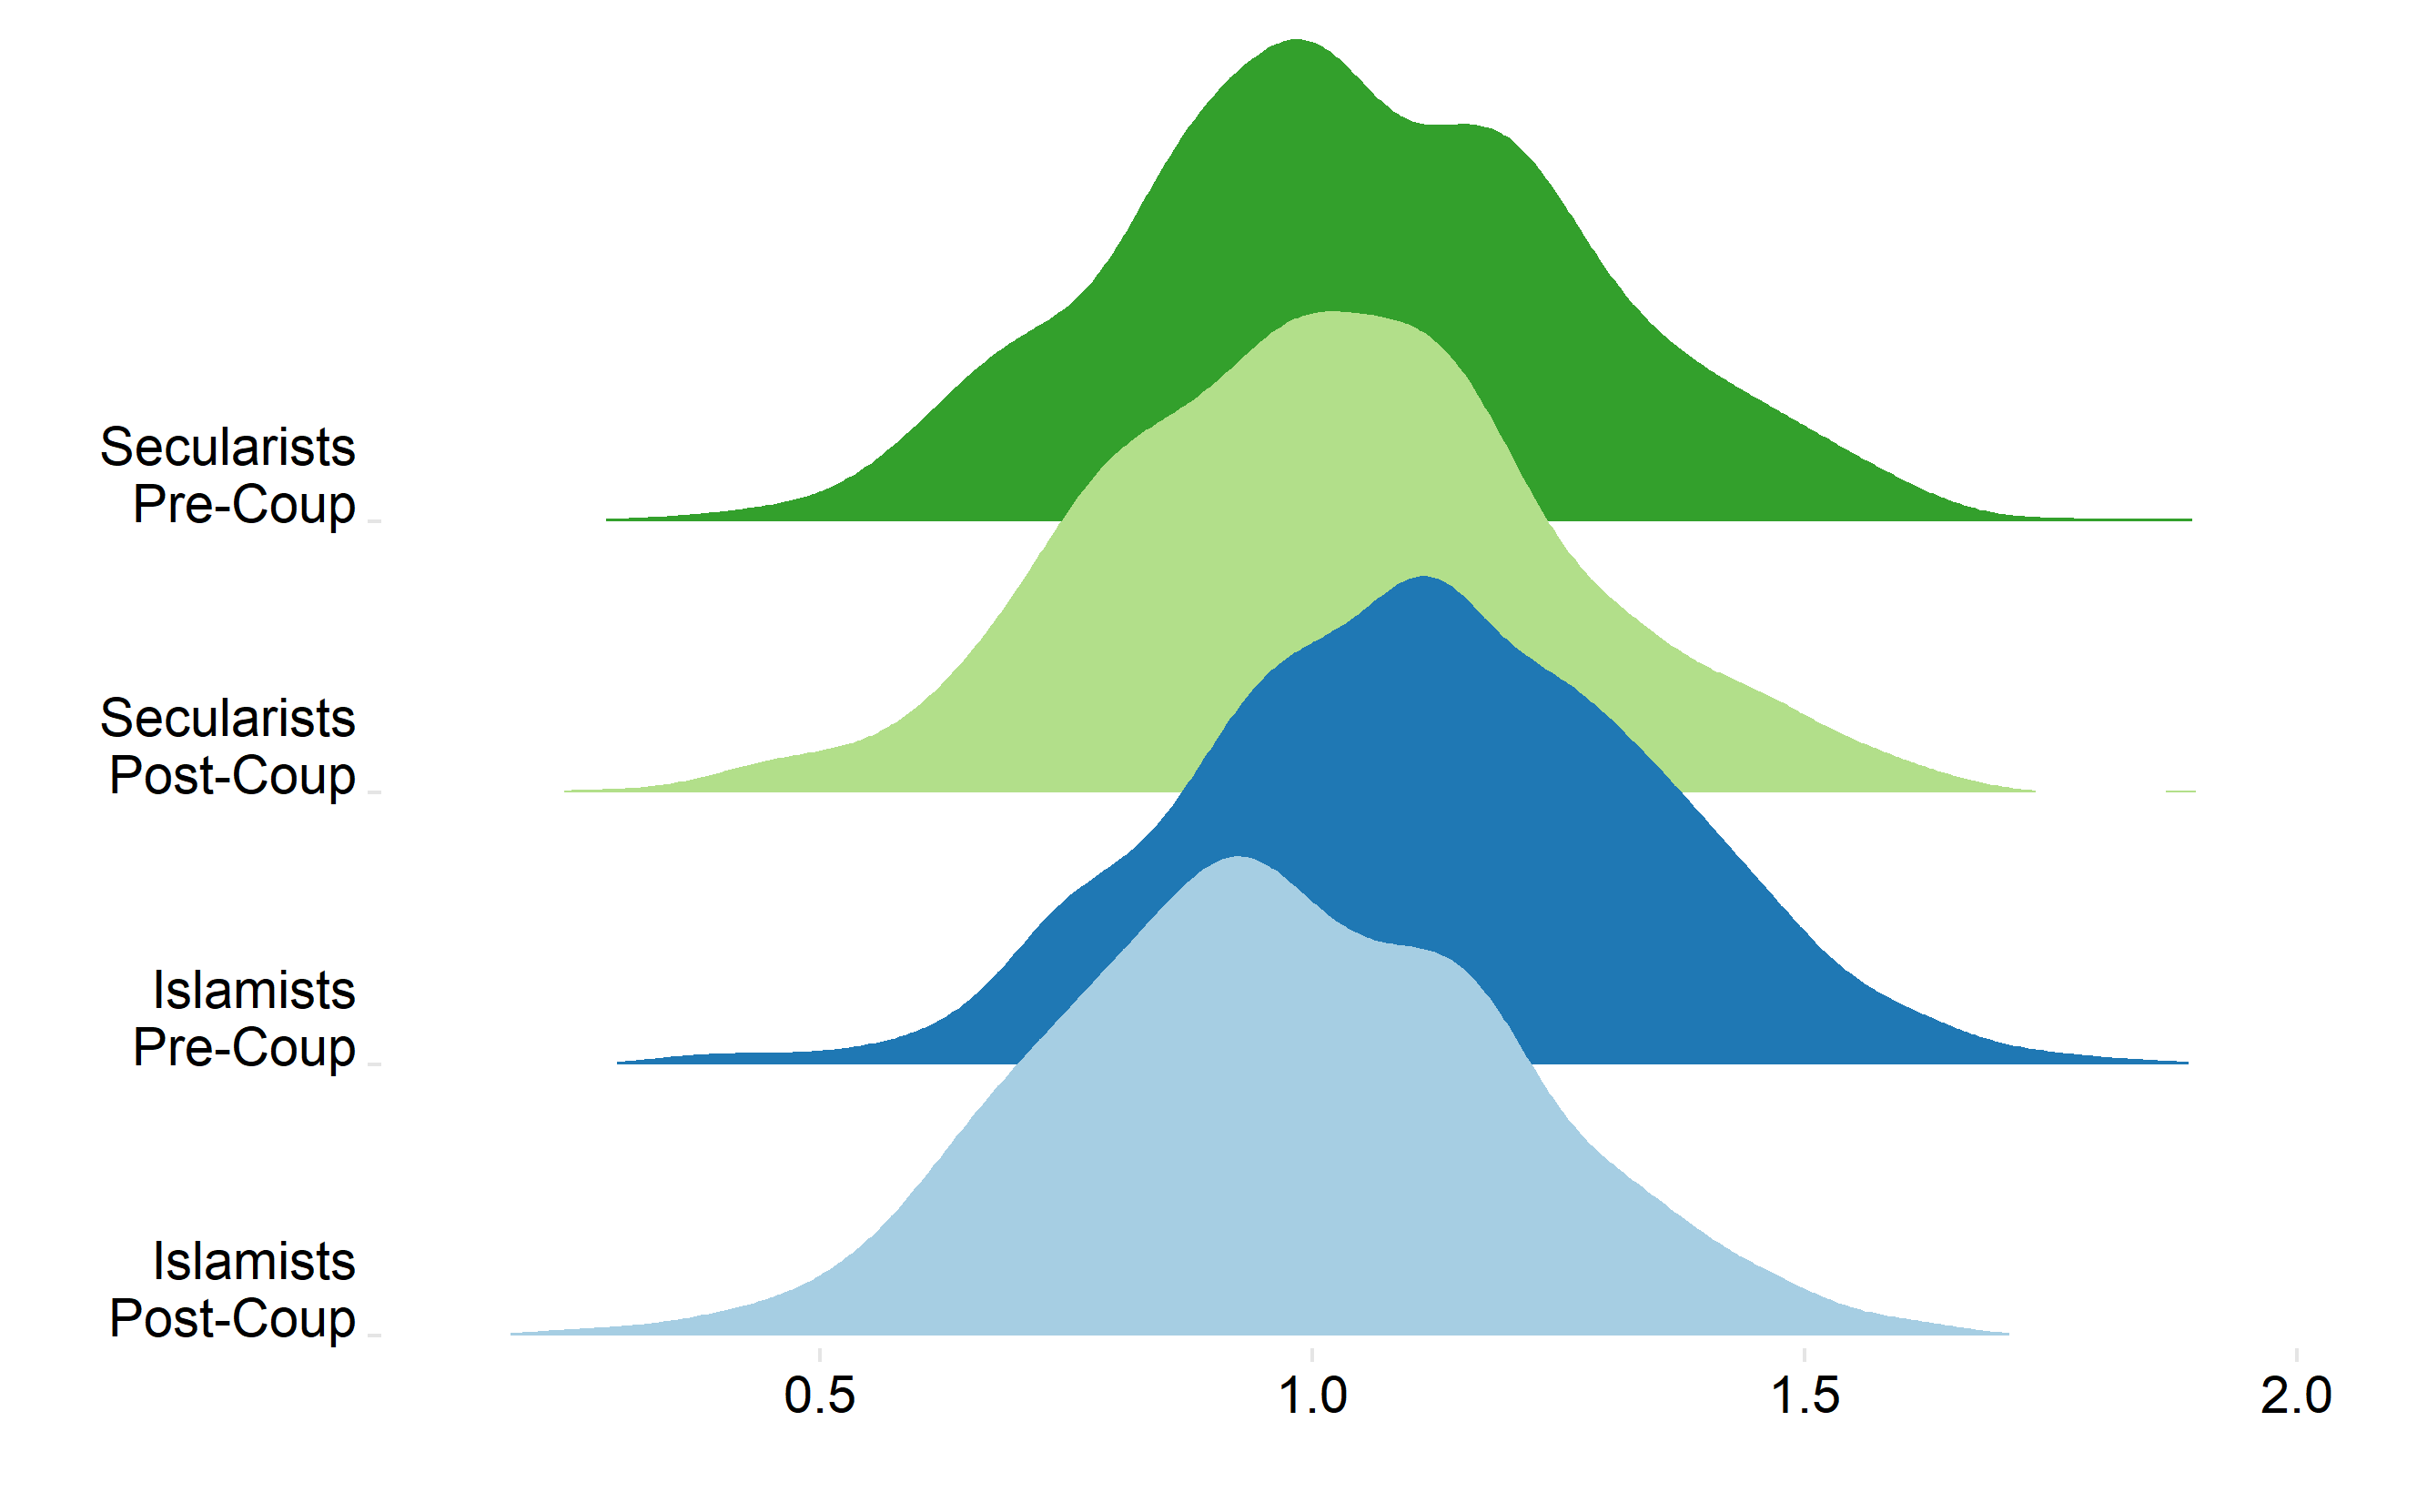
\includegraphics[width=.9\linewidth]{adj_joy}
\end{figure}
	
We are limited in what we can learn from the $\gamma_g$ and co-integration vectors because these parameters pool over the entire time series while the shock is isolated to a few time periods of interest. Instead, we can use impulse-response functions (IRFs) to examine the extent to which ideal-point shocks transfer from one country to another. IRFs are the best way to assess this difference as they provide a precise estimate of the actual level of shock that transfers from one time series to another along with an estimate of the decay in that shock over time. We estimate a two-standard deviation shock, which corresponds to 0.5 on the ideal point scale, first on the Tunisian time series and then on the Egyptian time series. 

Figures \ref{irf_tunis} and \ref{irf_egypt} show the decay function of this shock on ideal points among ideological groups in the other country. As can be seen, even though $\gamma_g$ values do not change dramatically post-coup, the level of shock transfer is higher. For Islamists in both countries, a two-standard deviation shock in their ideal points transmits about one-tenth of its force to their co-religionists. For secularists, these values are lower and amount to approximately five percent of the shock transferring. Furthermore, these shocks last up to six periods, or nearly 18 days, which is a significant period of time. It is interesting to note the peculiar shape of the pre-coup IRF for Islamists. This oscillating curve may denote that feedback was leading the Islamists in an upward trajectory, as can be seen in the ideal point graphs in Figure \ref{arab_id_facet}.
 \begin{figure}[!h]
	\centering
	\caption{IRF for Two-SD Shock from Tunisia to Egypt}\label{irf_tunis}
	\centering
	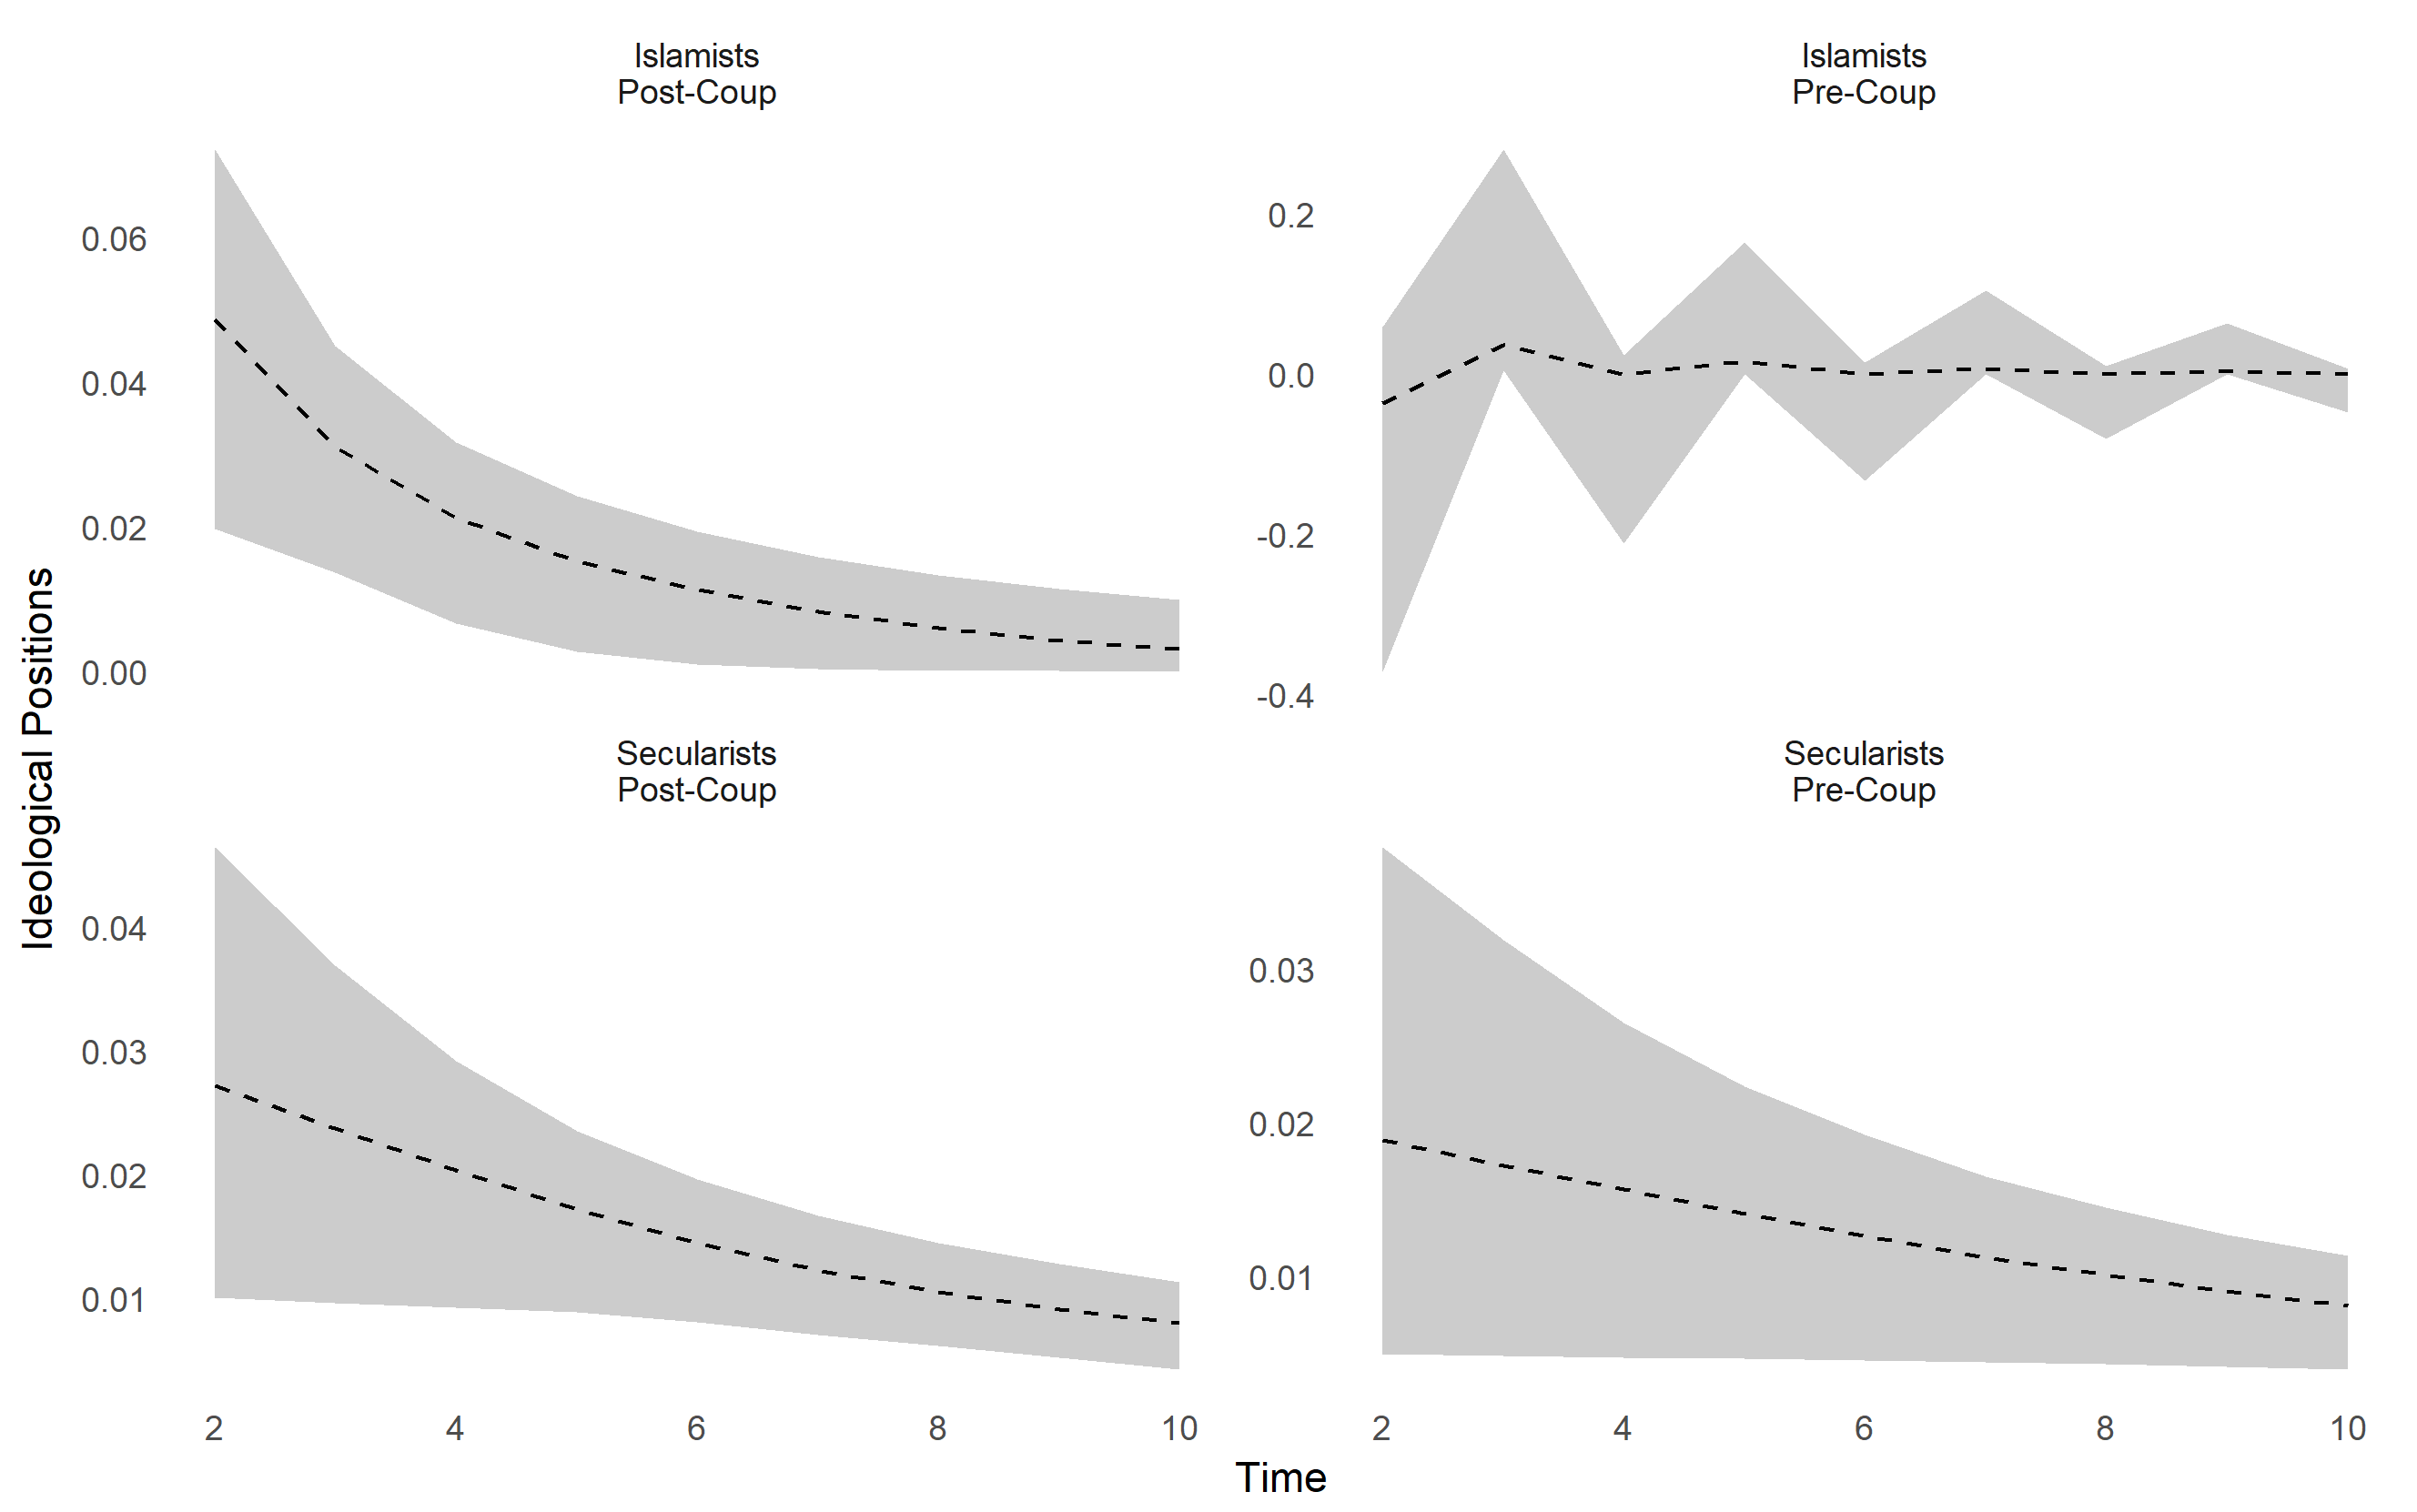
\includegraphics[width=.9\linewidth]{irf_tunisia}
\end{figure}
 \begin{figure}[!h]
	\centering
	\caption{IRF for Two-SD Shock from Egypt to Tunisia}\label{irf_egypt}
	\centering
	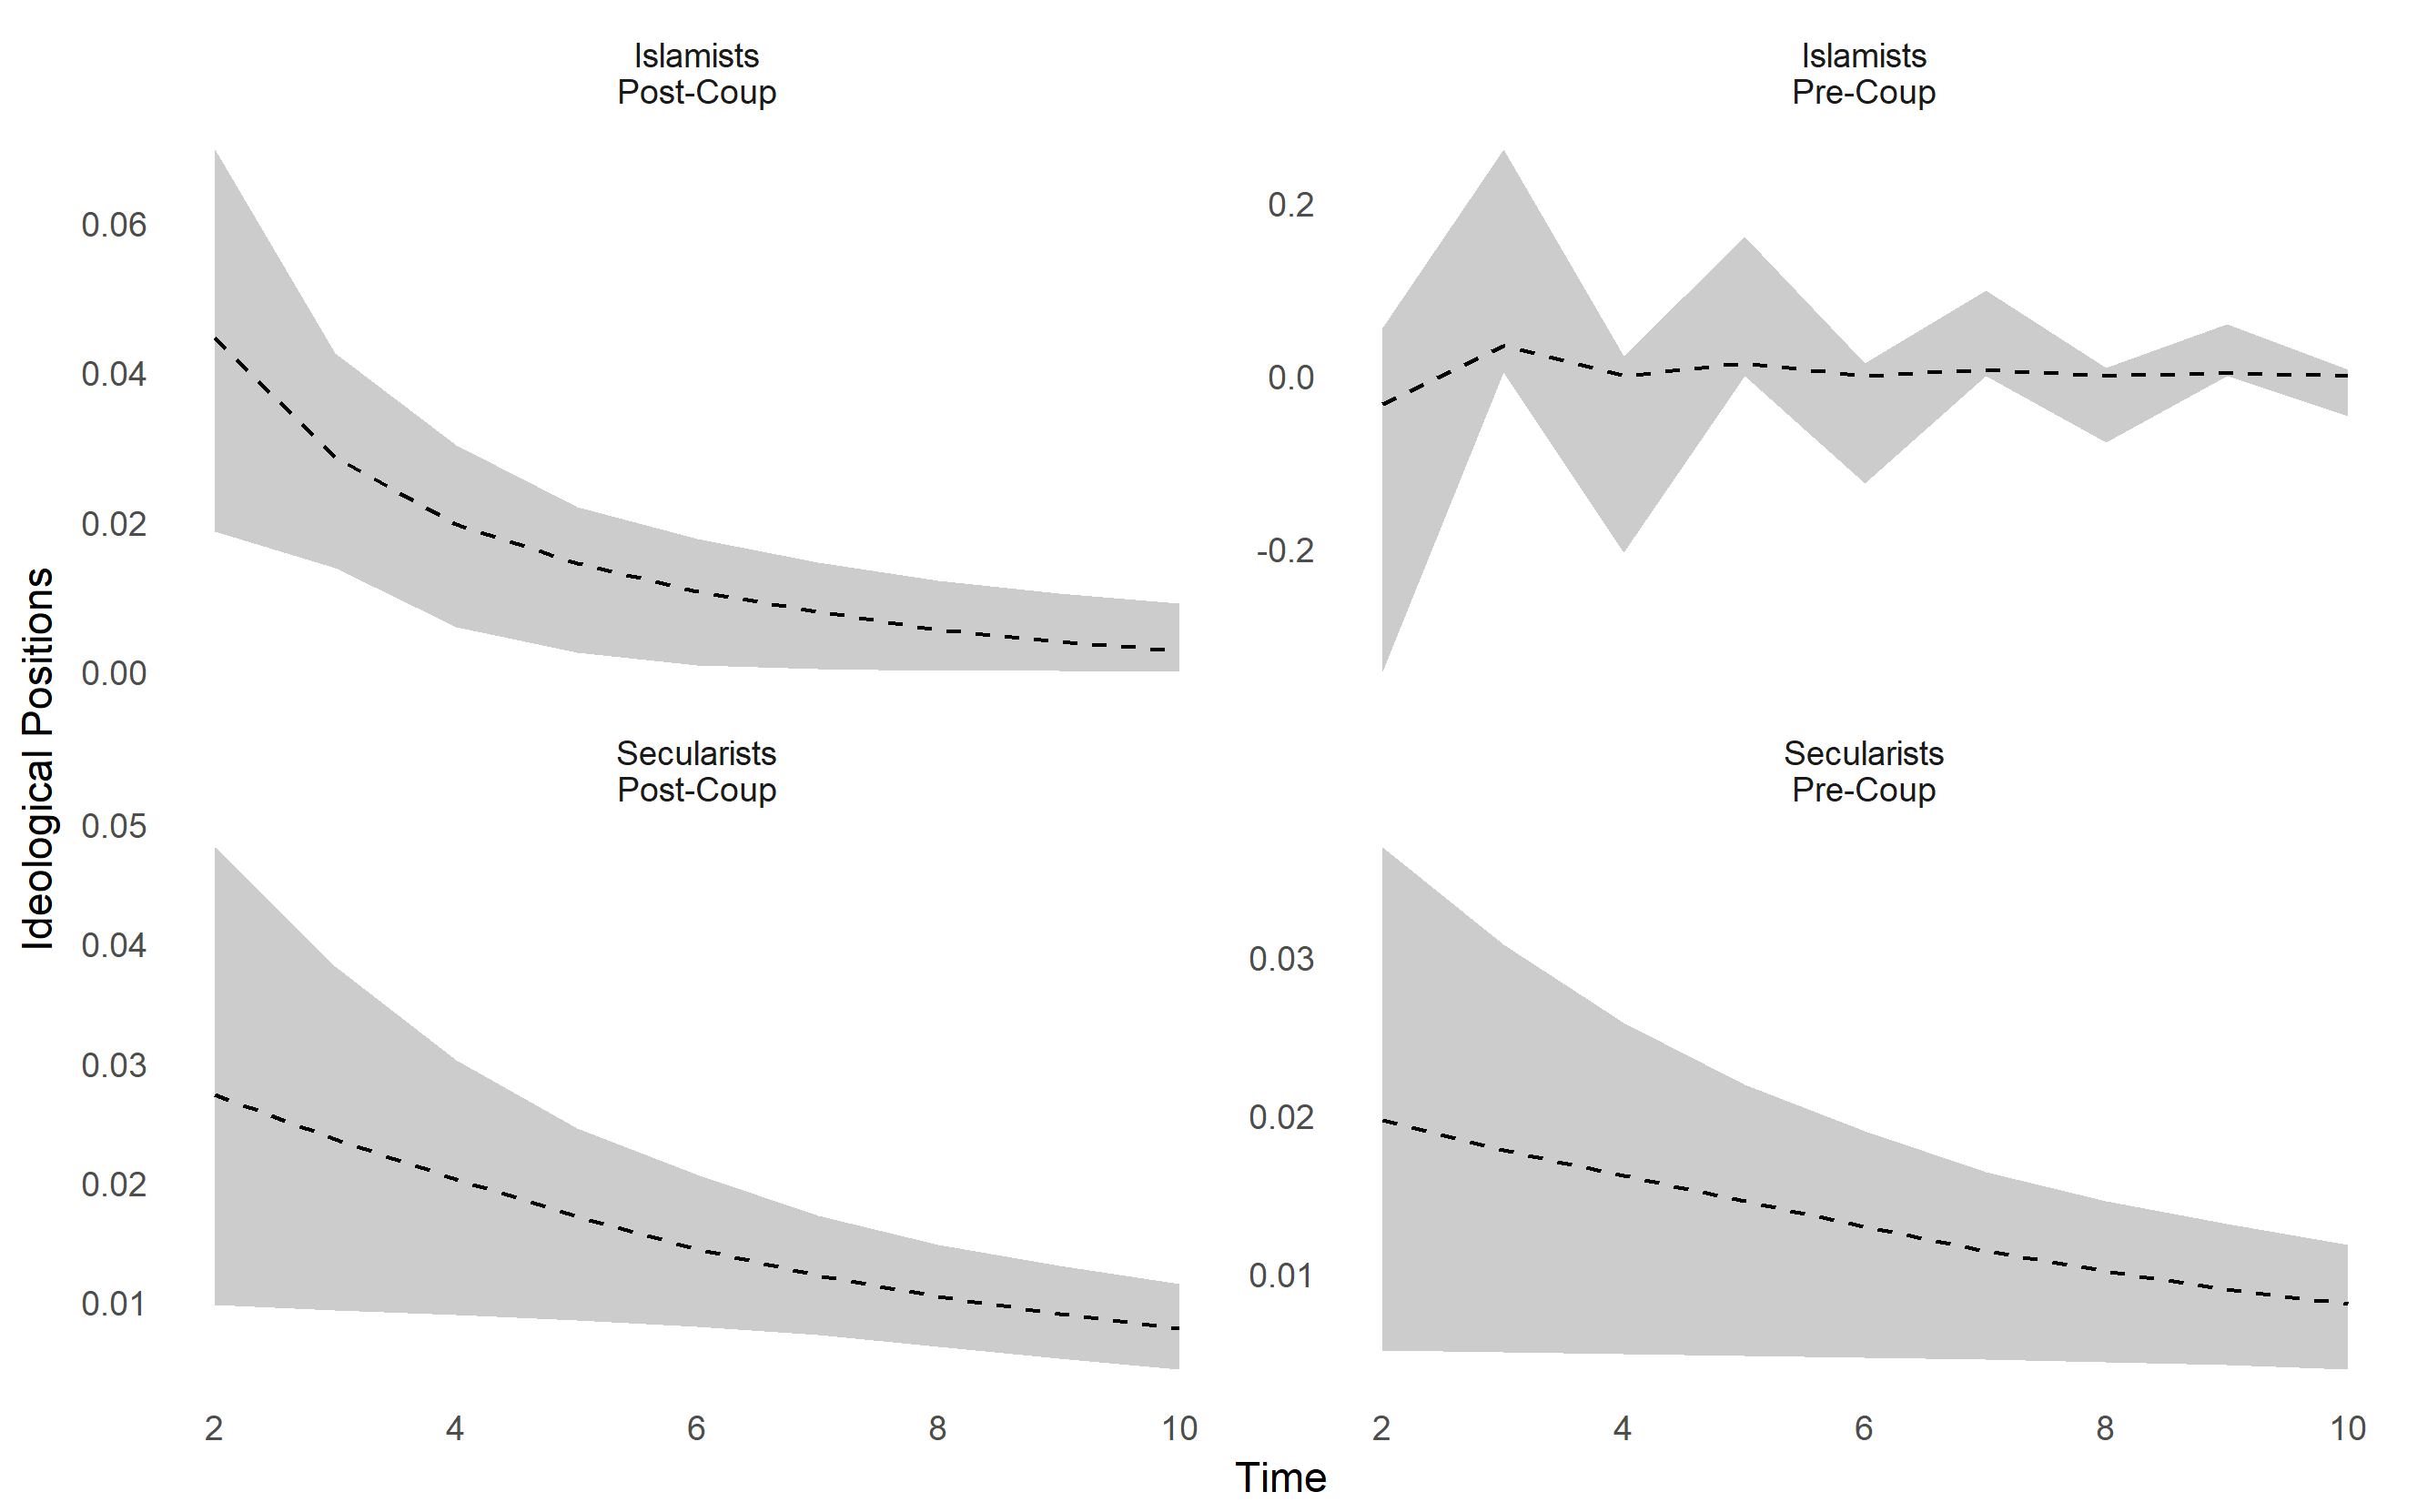
\includegraphics[width=.9\linewidth]{irf_egypt}
\end{figure}

Given the limited variation and precision of the $\gamma_g$ statistics and the co-integrating vectors, our best evidence for hypothesis 3 concerning cross-national polarization are the IRFs which appear to show higher levels of inclusion of shocks across countries after the coup. Given that these are initial estimates, we cannot compare these estimates with extant literature describing what a high level of transfer would be in this data, but we believe that a ten-percent transfer of shock represents a sizable connection between Islamists across countries. Furthermore, we can say with reasonable confidence that Islamists are more likely to track each other than secularists are in our sample.

\section*{Discussion}

Because both the model, theory and data in this paper are novel, the outcomes of the model should be treated as initial estimates of the phenomena of interest. While Twitter has been used to measure polarization \parencite{jamaletal2015,hu2012lda}, the use of latent ideological scores and time-series dynamics provides a direct estimate of the polarization of specific groups over time while still accounting for measurement uncertainty. This novelty, however, makes it difficult to situate these results without comparable studies to provide an indication as to whether a ten-percent transfer in shocks should be considered large or moderate during a politically-turbulent period. Thus as is often the case, the increase in measurement precision also generates new hypotheses and areas for exploration.

This study is further limited by the time range under consideration, approximately nine months during a period of political instability in the Arab Spring. As we described in our theory section, endogenous polarization occurs within and between countries over time, so it can be difficult to obtain a long enough series to show all of the polarizing effects and their consequential after-shocks. For our data, we are limited in modeling dynamics before 2012 because many of the Islamists did not open Twitter accounts until the beginning of 2013, leaving limited ideological diversity prior to that date. However, we may be able to gain more leverage on the long-term effects of polarizing events by extending our data collection on through 2014 and even the present.

In terms of modeling, it is apparent that it would be useful to try to look at how summary statistics such as the $\gamma_g$ parameters themselves vary over time. Adding yet another dimension to an already complicated model, however, may be challenging. We can consider adding some kind of smoothing prior over $\gamma_g$ to allow for some variation over time while still being able to have stable estimation. One possibility is to explore the use of Gaussian regression priors for these coefficients \parencite{rasmussen2006}.

Second, we can also explore models that incorporate an explicit second-dimension of the pro and anti-democracy axis, perhaps through the use of compensatory multi-dimensional IRT \parencite{reckase2009}. Doing so, however, would involve estimating two sets of time-series for each ideological group, and then allowing both sets of time-series to interact with their ideological counter-parts in other states. This approach may simply be too complicated to be of much use in this situation. Another approach is to consider differential item functioning (DIF) in which we allow the ideal points of the citizens to interact with an indicator for whether the elites are pro-democratic or anti-democratic \parencite{jackman2004}. 

Finally, we would note that the time series estimates may also be affected by de-polarization. In Tunisia, Islamists were under considerable pressure during this time period as they faced rising unrest because of violence from Islamic radicals \parencite{mccarthy2016}. For that reason, post-coup they may have feared supporting their co-religionists too publicly lest they suffer a similar fate within their own country \parencite{grewal2016}. This kind of suppression is unfortunately difficult to separate from an actual finding of no relationship between ideological groups, although further analysis of the content of the tweets can provide an indication as to whether de-polarization was a strategy pursued by Islamists in Tunisia.

\section*{Conclusion}

In this paper we put forward a method of estimating the latent positions of ideological groups in Egypt and Tunisia during the tumultuous period of the Arab Spring. We take advantage of Twitter's widespread usage to show how latent ideological scores change over time and also in tandem with similar ideological groups in other countries. The use of IRT models allows for these estimates to incorporate measurement uncertainty while also providing useful summary measures of ideological position.

We find that the overthrow of Mohammed Morsi in a coup by the Egyptian military resulted in a dramatic swing of the ideal points of both secularists and Islamists in Egypt. This shock also eventually resulted in both groups moving farther apart from each other in the months ahead. In the specific aftermath of the coup, we find only limited evidence of rapid polarization in Tunisia, although over time we find that the relationship between Islamists in Tunisia and Egypt grew stronger. After Morsi's coup, approximately ten percent of change in the ideological position of Islamists caused change in the ideological position of Tunisian Islamists. Furthermore, we find that secularists within both countries began to follow each other more closely after the coup.

This research opens the door to further exploration of the determinants and measurement of ideological polarization during periods of political instability. This model provides a rich range of estimates and can pinpoint places at which polarizing events occurred. Furthermore, we can show how short-term shocks translate into long-term differences in idealogical polarization over time. We hope that this evidence stimulates more investigation of the determinants and effects of group feedback effects in ideologically-polarized societies.

\section*{Appendix: List of Elites}

\begin{longtable}{rllll}
	\hline
	& Username & Secularist/Islamist & Pro/Anti Democracy & Country \\ 
	\hline
	1 & slim404 & Secularist & Pro Dem. & Tunisia \\ 
	2 & ooouups & Secularist & Pro Dem. & Tunisia \\ 
	3 & nawaat & Secularist & Pro Dem. & Tunisia \\ 
	4 & psycke & Secularist & Pro Dem. & Tunisia \\ 
	5 & karim2k & Secularist & Pro Dem. & Tunisia \\ 
	6 & riadheh & Secularist & Pro Dem. & Tunisia \\ 
	7 & mira404 & Secularist & Pro Dem. & Tunisia \\ 
	8 & yassayari & Secularist & Pro Dem. & Tunisia \\ 
	9 & ka33boura & Secularist & Pro Dem. & Tunisia \\ 
	10 & sarah\_bh & Secularist & Pro Dem. & Tunisia \\ 
	11 & majdikhan & Secularist & Pro Dem. & Tunisia \\ 
	12 & maramirou & Secularist & Pro Dem. & Tunisia \\ 
	13 & marwen & Secularist & Pro Dem. & Tunisia \\ 
	14 & benmhennilina & Secularist & Pro Dem. & Tunisia \\ 
	15 & slimazzabi & Islamist & Pro Dem. & Tunisia \\ 
	16 & jnayna & Secularist & Pro Dem. & Tunisia \\ 
	17 & azyyoz & Secularist & Pro Dem. & Tunisia \\ 
	18 & arabasta1 & Secularist & Pro Dem. & Tunisia \\ 
	19 & zinga\_ & Secularist & Pro Dem. & Tunisia \\ 
	20 & c\_moii & Secularist & Pro Dem. & Tunisia \\ 
	21 & jasmintn & Secularist & Pro Dem. & Tunisia \\ 
	22 & sans\_url & Secularist & Anti Dem. & Tunisia \\ 
	23 & indigo\_light & Islamist & Pro Dem. & Tunisia \\ 
	24 & takriz & Secularist & Pro Dem. & Tunisia \\ 
	25 & sameh\_b & Secularist & Pro Dem. & Tunisia \\ 
	26 & nayzek & Secularist & Pro Dem. & Tunisia \\ 
	27 & liliopatra & Secularist & Pro Dem. & Tunisia \\ 
	28 & eyaturki & Secularist & Pro Dem. & Tunisia \\ 
	29 & faiyla & Secularist & Pro Dem. & Tunisia \\ 
	30 & zizoo & Secularist & Pro Dem. & Tunisia \\ 
	31 & amal\_haouet & Islamist & Pro Dem. & Tunisia \\ 
	32 & houeida & Islamist & Pro Dem. & Tunisia \\ 
	33 & malekk & Secularist & Pro Dem. & Tunisia \\ 
	34 & ahlemhc & Secularist & Anti Dem. & Tunisia \\ 
	35 & tom\_z & Secularist & Anti Dem. & Tunisia \\ 
	36 & chiheb12 & Secularist & Pro Dem. & Tunisia \\ 
	37 & al\_pacino\_ & Secularist & Pro Dem. & Tunisia \\ 
	38 & zeinebturki & Secularist & Pro Dem. & Tunisia \\ 
	39 & khamousss & Secularist & Pro Dem. & Tunisia \\ 
	40 & may\_mouna & Secularist & Pro Dem. & Tunisia \\ 
	41 & yamenbousrih & Secularist & Anti Dem. & Tunisia \\ 
	42 & ifikra & Secularist & Pro Dem. & Tunisia \\ 
	43 & r\_ghannouchi & Islamist & Pro Dem. & Tunisia \\ 
	44 & nahdhatunisie & Islamist & Pro Dem. & Tunisia \\ 
	45 & ali\_larayedh & Islamist & Pro Dem. & Tunisia \\ 
	46 & yusraghkh & Islamist & Pro Dem. & Tunisia \\ 
	47 & ziedladhari & Islamist & Pro Dem. & Tunisia \\ 
	48 & bassemloukil & Secularist & Anti Dem. & Tunisia \\ 
	49 & mehdi\_jomaa & Secularist & Anti Dem. & Tunisia \\ 
	50 & jasminef\_tn & Islamist & Pro Dem. & Tunisia \\ 
	51 & alaa & Secularist & Pro Dem. & Egypt \\ 
	52 & waelabbas & Secularist & Pro Dem. & Egypt \\ 
	53 & ghonim & Secularist & Pro Dem. & Egypt \\ 
	54 & nawaranegm & Secularist & Pro Dem. & Egypt \\ 
	55 & sandmonkey & Secularist & Pro Dem. & Egypt \\ 
	56 & elbaradei & Secularist & Pro Dem. & Egypt \\ 
	57 & zeinobia & Secularist & Pro Dem. & Egypt \\ 
	58 & 3arabawy & Secularist & Pro Dem. & Egypt \\ 
	59 & amrmsalama & Secularist & Pro Dem. & Egypt \\ 
	60 & monasosh & Secularist & Pro Dem. & Egypt \\ 
	61 & kalimakhus & Secularist & Pro Dem. & Egypt \\ 
	62 & drbassemyoussef & Secularist & Pro Dem. & Egypt \\ 
	63 & belalfadl & Secularist & Pro Dem. & Egypt \\ 
	64 & gamaleid & Secularist & Pro Dem. & Egypt \\ 
	65 & salmaeldaly & Secularist & Pro Dem. & Egypt \\ 
	66 & yosrifouda & Secularist & Pro Dem. & Egypt \\ 
	67 & wael & Secularist & Pro Dem. & Egypt \\ 
	68 & monaeltahawy & Secularist & Pro Dem. & Egypt \\ 
	69 & alyaagad & Secularist & Pro Dem. & Egypt \\ 
	70 & galalamer & Secularist & Pro Dem. & Egypt \\ 
	71 & amrwaked & Secularist & Pro Dem. & Egypt \\ 
	72 & mand0z & Secularist & Pro Dem. & Egypt \\ 
	73 & adel\_salib & Secularist & Pro Dem. & Egypt \\ 
	74 & hazem\_azim & Secularist & Pro Dem. & Egypt \\ 
	75 & ahmadesseily & Secularist & Pro Dem. & Egypt \\ 
	76 & zeinabsamir & Secularist & Pro Dem. & Egypt \\ 
	77 & lilianwagdy & Islamist & Pro Dem. & Egypt \\ 
	78 & 5orm & Secularist & Pro Dem. & Egypt \\ 
	79 & sarahcarr & Secularist & Pro Dem. & Egypt \\ 
	80 & gsquare86 & Secularist & Pro Dem. & Egypt \\ 
	81 & minazekri & Secularist & Pro Dem. & Egypt \\ 
	82 & ahmednaguib & Secularist & Anti Dem. & Egypt \\ 
	83 & gemyhood & Islamist & Pro Dem. & Egypt \\ 
	84 & shokeir & Secularist & Pro Dem. & Egypt \\ 
	85 & heshoz & Secularist & Anti Dem. & Egypt \\ 
	86 & mennagamal & Islamist & Pro Dem. & Egypt \\ 
	87 & theboghdady & Secularist & Pro Dem. & Egypt \\ 
	88 & seksek & Secularist & Pro Dem. & Egypt \\ 
	89 & sarahngb & Secularist & Pro Dem. & Egypt \\ 
	90 & thebigpharaoh & Secularist & Pro Dem. & Egypt \\ 
	91 & h\_eid & Secularist & Pro Dem. & Egypt \\ 
	92 & lastoadri & Secularist & Pro Dem. & Egypt \\ 
	93 & rashapress & Secularist & Pro Dem. & Egypt \\ 
	94 & minanaguib90 & Secularist & Pro Dem. & Egypt \\ 
	95 & ahmad\_khalil & Secularist & Pro Dem. & Egypt \\ 
	96 & naguibsawiris & Secularist & Pro Dem. & Egypt \\ 
	97 & mazloum & Secularist & Pro Dem. & Egypt \\ 
	98 & nabilelhalfawy & Secularist & Pro Dem. & Egypt \\ 
	99 & theadly & Secularist & Pro Dem. & Egypt \\ 
	100 & thesherio & Secularist & Pro Dem. & Egypt \\ 
	101 & kalnaga & Secularist & Pro Dem. & Egypt \\ 
	102 & dr\_heba\_raouf & Secularist & Pro Dem. & Egypt \\ 
	103 & moftasa & Secularist & Pro Dem. & Egypt \\ 
	104 & ahmdalish & Secularist & Pro Dem. & Egypt \\ 
	105 & theonlywarman & Secularist & Pro Dem. & Egypt \\ 
	106 & pakinamamer & Secularist & Pro Dem. & Egypt \\ 
	107 & zelaky & Islamist & Pro Dem. & Egypt \\ 
	108 & embee & Secularist & Pro Dem. & Egypt \\ 
	109 & ahmada2 & Secularist & Pro Dem. & Egypt \\ 
	110 & ramiii & Secularist & Pro Dem. & Egypt \\ 
	111 & mar3e & Secularist & Pro Dem. & Egypt \\ 
	112 & alaaaswany & Secularist & Pro Dem. & Egypt \\ 
	113 & alienzero & Secularist & Pro Dem. & Egypt \\ 
	114 & salmasaid & Secularist & Pro Dem. & Egypt \\ 
	115 & i3atef & Secularist & Pro Dem. & Egypt \\ 
	116 & loainagati & Secularist & Pro Dem. & Egypt \\ 
	117 & memam8 & Secularist & Pro Dem. & Egypt \\ 
	118 & ayaabdullah & Secularist & Pro Dem. & Egypt \\ 
	119 & bassem\_sabry & Secularist & Pro Dem. & Egypt \\ 
	120 & bothainakamel1 & Secularist & Pro Dem. & Egypt \\ 
	121 & tarekshalaby & Secularist & Pro Dem. & Egypt \\ 
	122 & m3adel & Secularist & Pro Dem. & Egypt \\ 
	123 & malek & Secularist & Pro Dem. & Egypt \\ 
	124 & etharkamal & Islamist & Pro Dem. & Egypt \\ 
	125 & ssirgany & Secularist & Pro Dem. & Egypt \\ 
	126 & \_\_safi\_\_ & Secularist & Pro Dem. & Egypt \\ 
	127 & hfakhry & Secularist & Pro Dem. & Egypt \\ 
	128 & hamzanamira & Secularist & Pro Dem. & Egypt \\ 
	129 & asmaamahfouz & Secularist & Pro Dem. & Egypt \\ 
	130 & egyptocracy & Secularist & Pro Dem. & Egypt \\ 
	131 & nasry & Secularist & Pro Dem. & Egypt \\ 
	132 & themiinz & Islamist & Pro Dem. & Egypt \\ 
	133 & muhammadmorsi & Islamist & Pro Dem. & Egypt \\ 
	134 & ikhwanweb & Islamist & Pro Dem. & Egypt \\ 
	135 & mushaweh & Islamist & Pro Dem. & Egypt \\ 
	136 & azzaelgarf & Islamist & Pro Dem. & Egypt \\ 
	137 & asmaaghazalll & Islamist & Pro Dem. & Egypt \\ 
	138 & alnourpartyeg & Islamist & Anti Dem. & Egypt \\ 
	139 & yonosmakhyoun & Islamist & Anti Dem. & Egypt \\ 
	140 & naderbakkar & Islamist & Pro Dem. & Egypt \\ 
	141 & gelhaddad & Islamist & Pro Dem. & Egypt \\ 
	142 & alqaradawy & Islamist & Pro Dem. & Egypt \\ 
	\hline
	\hline
\end{longtable}

\printbibliography






\end{document}